\documentclass[titlepage]{article}
\usepackage{amsmath}
\usepackage{amssymb}
\usepackage{indentfirst}
\usepackage[margin=1in]{geometry}
\usepackage{longtable}
\usepackage{enumitem}
\usepackage{fancyvrb}
%\usepackage{graphicx}
\usepackage{pdfpages}
\usepackage{subcaption}
\usepackage{flafter}
\usepackage[section]{placeins}
\usepackage{float}
\hyphenation{wave-guide}
\renewcommand\_{\textunderscore\linebreak[1]}

\begin{document}

\begin{titlepage}

   \centering
   \vspace*{3cm}
   {\huge\bfseries OpenParEM2D Theory, Methodology, and Accuracy} \\
   \vskip1cm
   {\Large Version 2.1} \\
   \vskip1cm
   {\Large April 2025} \\
   \vskip1cm
   {\Large Brian Young} \\

   \vfill

   \includegraphics[width=0.5\textwidth]{figures/logo-crop}

   \vspace*{\fill}
   Copyright \copyright{} 2025 Brian Young. All Rights Reserved.
\end{titlepage}

\tableofcontents

\newpage
\section{Introduction}

OpenParEM2D is a full-wave electromagnetic solver using the finite-element method to solve for the frequency-dependent complex propagation constant, fields, and characteristic impedance for the dominant and optionally higher-order modes for transmission lines and waveguides.  The Galerkin procedure is applied to Maxwell's equations to derive the weak form of the wave equation in $\overline{E}$ which is then specialized for transmission lines and waveguides by assuming that the z-dependence in the direction of propagation is restricted to $e^{-\gamma z}$, where $\gamma$ is the complex propagation constant.  The integrals are calculated with calls to the MFEM library \cite{MFEM}\cite{MFEMweb}, boundary conditions are applied, and finally the generalized complex eigenvalue problem given as $\overline{\overline{A}}\,\overline{x}=\lambda\overline{\overline{B}}\,\overline{x}$ is solved for $\gamma$ and $\overline{E}$.  Post-processing calculates the magnetic field $\overline{H}$, power, characteristic impedance, and a loss adder for surface impedances.  The methodology uses fully populated matrices, so OpenParEM2D is not configured for GPU processing.

Boundary conditions include perfect magnetic conductor (PMC), perfect electric conductor (PEC), and surface impedance.  The default boundary condition for all edges facing voids is PEC.  Edges facing voids can be set to PMC or surface impedance.  Losses due to surface impedances are calculated from the $\overline{H}$ and added to the dielectric losses, which are calculated as part of the eigenvalue solution.

This document covers the theory and methodology of how OpenParEM2D builds and solves the eigenvalue problem along with post-processing calculations.  Accuracy is demonstrated with a number of test cases.  For details about how to set up and run OpenParEM2D, see the separate document "OpenParEM2D\_Users\_Manual.pdf".

\section{Theory and Mapping to MFEM}

\subsection{Wave Equation}

The methodology of OpenParEM2D follows that of \cite{Lee}.  For completeness and clarity, the entire methodology is re-derived here. 

Starting at the most fundamental level with Maxwell's equations, we have
\begin{equation}
\label{eq:faraday}
\nabla\times\overline{E}=-\text{j}\omega\mu\overline{H}
\end{equation}
and
\begin{equation}
\label{eq:ampere}
\nabla\times\overline{H}=\overline{J}+\text{j}\omega\epsilon\overline{E}.
\end{equation}
Let $\overline{J}=\sigma\overline{E}$ and $\epsilon_c=\frac{\sigma}{\text{j}\omega}+\epsilon$, then (\ref{eq:ampere}) becomes
\begin{equation}
\label{eq:ampere2}
\nabla\times\overline{H}=\text{j}\omega\epsilon_c\overline{E}.
\end{equation}
Eliminating $\overline{H}$ from (\ref{eq:ampere2}) and (\ref{eq:faraday}) yields 
\begin{equation}
\nabla\times(-\frac{1}{\text{j}\omega\mu}\nabla\times\overline{E})=\text{j}\omega\epsilon_c\overline{E}.
\end{equation}
Multiply through by $\text{j}\omega\mu_\circ$ and set $k_\circ^2=\omega^2\mu_\circ\epsilon_\circ$ to get the wave equation
\begin{equation}
\label{eq:wave_equation}
\nabla\times(\frac{1}{\mu_r}\nabla\times\overline{E})=k_\circ^2\epsilon_{cr}\overline{E},
\end{equation}
where $\epsilon_{cr}=\epsilon_c/\epsilon_\circ$ and $\mu_r=\mu/\mu_{\circ}$.

\subsection{Galerkin's Procedure}

Multiply (\ref{eq:wave_equation}) by a test field $\overline{T}$ and integrate over the volume, $\Omega$, to get 
\begin{equation}
\iiint_{\Omega}\nabla\times(\frac{1}{\mu_r}\nabla\times\overline{E})\cdot\overline{T}dV=\iiint_{\Omega} k_\circ^2\epsilon_{cr}\overline{E}\cdot\overline{T}dV.
\end{equation}
The surface of $\Omega$ is designated by $\delta$.  Conventionally, the normal to the volume at the surface is given by $\hat{n}$, which points out of the 3D volume.  Apply the vector identity
\begin{equation}
\iiint_{\Omega}\nabla\times\overline{u}\cdot\overline{v}\,d\Omega=\iiint_{\Omega}\overline{u}\cdot\nabla\times\overline{v}\,d\Omega-\iint_{\delta}(\overline{u}\times\hat{n})\cdot\overline{v}\,dS
\end{equation}
with $\overline{u}=\frac{1}{\mu_r}\nabla\times\overline{E}$ and $\overline{v}=\overline{T}$ and rearranging, then
\begin{equation}
\iiint_{\Omega}\frac{1}{\mu_r}\nabla\times\overline{E}\cdot\nabla\times\overline{T}\,dV-k_\circ^2\iiint_{\Omega}\epsilon_{cr}\overline{E}\cdot\overline{T}dV-\iint_{\delta}(\frac{1}{\mu_r}\nabla\times\overline{E}\times\hat{n})\cdot\overline{T}\,dS=0.
\end{equation}
Reorder the cross products involving $\hat{n}$ to get the weak form of the wave equation in $\overline{E}$ as
\begin{equation}
\label{eq:weak_form}
\iiint_{\Omega}\frac{1}{\mu_r}\nabla\times\overline{E}\cdot\nabla\times\overline{T}\,dV-k_\circ^2\iiint_{\Omega}\epsilon_{cr}\overline{E}\cdot\overline{T}dV+\iint_{\delta}\hat{n}\times(\frac{1}{\mu_r}\nabla\times\overline{E})\cdot\overline{T}\,dS=0,
\end{equation}
which has two terms over the volume and one over the surface. 

\subsection{Specialization for Transmission Lines and Waveguides}
\label{sec:specialization}

Eq.~\ref{eq:weak_form} is general for 3D spaces, but for transmission lines and waveguides, the 3D problem is specialized as an electromagnetic field on a 2D surface in the x-y plane that changes in the z-direction only with the dependence $e^{-\gamma z}$. With this z-dependence, $\frac{\partial}{\partial z}\rightarrow -\gamma$. Following \cite{Lee}, the electric field can be written in terms of its transverse and longitudinal components as
\begin{equation}
\overline{E}=\overline{E}_t+E_z\hat{z}.
\end{equation} 
as well as the operator
\begin{equation}
\nabla=\nabla_t+\frac{\partial}{\partial z}\hat{z}=\nabla_t-\gamma\hat{z}.
\end{equation}
Substituting these into (\ref{eq:weak_form}) and equating the transverse components (t) yields
\begin{equation}
\label{eq:transverse1}
\nabla_t\times\frac{1}{\mu_r}\nabla_t\times\overline{E}_t-\gamma^2\frac{1}{\mu_r}\overline{E}_t-\gamma\frac{1}{\mu_r}\nabla_t E_z=k_{\circ}^2 \epsilon_{cr}\overline{E}_t
\end{equation}
while matching the longitudinal (z) components yields
\begin{equation}
\label{eq:longitudinal1}
\nabla_t\cdot\frac{1}{\mu_r}\nabla_t E_z+\frac{1}{\mu_r}\gamma\nabla_t\cdot\overline{E}_t+k_{\circ}^2\epsilon_{cr}E_z=0.
\end{equation}

An issue with (\ref{eq:transverse1}) is the presence of both $\gamma$ and $\gamma^2$.  The targeted generalized eigenvalue equation form is $\overline{\overline{A}}\,\overline{x}=\lambda\overline{\overline{B}}\,\overline{x}$, so a reformulation is needed.  Per \cite{Lee}, this can be accomplished by a change in variable equating $\overline{e}_t=\gamma\overline{E}_t$ along with $e_z=E_z$ for notational consistency.  Multiplying through (\ref{eq:transverse1}) by $\gamma$ then making these substitutions results in
\begin{equation}
\label{eq:transverse2}
\nabla_t\times\frac{1}{\mu_r}\nabla_t\times\overline{e}_t-\gamma^2(\frac{1}{\mu_r}\overline{e}_t+\frac{1}{\mu_r}\nabla_t \, e_z)=k_{\circ}^2 \epsilon_{cr}\overline{e}_t
\end{equation}
and similarly for (\ref{eq:longitudinal1}) multiplying through by $\gamma^2$
\begin{equation}
\label{eq:longitudinal2}
\gamma^2(\nabla_t\cdot\frac{1}{\mu_r}\nabla_t \, e_z+\frac{1}{\mu_r}\nabla_t\cdot\overline{e}_t+k_{\circ}^2\epsilon_{cr}e_z)=0.
\end{equation}
Now (\ref{eq:transverse2}) and (\ref{eq:longitudinal2}) can be configured into a generalized eigenvalue problem of the form $\overline{\overline{A}}\,\overline{x}=\lambda\overline{\overline{B}}\,\overline{x}$ with $\lambda=\gamma^2$.  Once the eigenvalue problem is solved for the eigenvalues and eigenvectors, $\gamma$ is found from the square root of $\lambda$ and the fields are found by dividing the $\overline{e}_t$ portion of the eigenvector with $\gamma$ and carrying over the $e_z$ portion to $E_z$.  

\subsection{Building the Eigenvalue Problem}

To build the standard generalized eigenvalue problem, (\ref{eq:transverse2}) and (\ref{eq:longitudinal2}) are converted to matrix form using finite elements with the the methods in the MFEM library.  Since the MFEM library is implemented only for real numbers, the methods must be called twice, once for the real part and once for the imaginary part, which are then combined into a complex matrix for solving as a complex eigenvalue problem.  For simplicity, the needed methods are noted here once, while OpenParEM2D implements the full complex calculation.  All of the operations are in the OpenParEM2D method \texttt{fem2D::fem2D}.

For the finite element implementation of the fields, the two variables are the vector $\overline{e}_t$ and the scalar $e_z$.  Different finite elements are needed to represent these since one is a vector and the other is a scalar.  For $\overline{e}_t$, Nedelec finite elements are used because they are vectors and because the divergence is zero, inherently satisfying Gauss's law assuming no free charge.  Use of Nedelec elements avoids spurious solutions.  For $e_z$, scalar H1 elements are used.

Both sets of finite elements are used on the same mesh to set up and solve the eigenvalue problem for $\overline{e}_t$ and $e_z$. The finite elements must be tracked, but for the most part, the MFEM library takes care of the details in structures called finite element spaces.

Finite elements implement mathematical operations using bilinear form integrators and mixed bilinear form integrators on finite element spaces.  For vector-to-vector operations, such as for the curl operator, MFEM uses bilinear form integrators on a single finite element space, resulting in a square matrix.
For vector-to-scalar and scalar-to-vector operations, such as the dot product (vector to scalar) and the gradient (scalar to vector), MFEM uses mixed bilinear form integrators on two finite element spaces, resulting in a non-square matrix.

The bilinear form integrators support element-by-element variation in the permittivity and permeability.  OpenParEM2D supports complex permittivity that can vary by regions, and by extension element-by-element.  For permeability, only real permeability is supported, but it can very by region.  Extension of OpenParEM2D to support complex permeability would require adding support for complex matrices similar to that used for the permittivity.  All materials are assumed to be isotropic, but the MFEM library does support extension to anisotropic materials.

Implementing the four terms of (\ref{eq:transverse2}) term-by-term, the first term is
\begin{equation}
\nabla_t\times\frac{1}{\mu_r}\nabla_t\times\overline{e}_t,
\end{equation}
and it is implemented by the MFEM CurlCurlIntegrator using a bilinear form integrator on the Nedelec finite element space.  Following the notation in \cite{Lee}, the resulting matrix is called $\overline{\overline{S}}_t$, and it multiplies $\overline{e}_t$.  The second term is 
\begin{equation}
\frac{1}{\mu_r}\overline{e}_t,
\end{equation}
which is implemented by MFEM's VectorFEMassIntegrator using a bilinear form integrator on the Nedelec finite element space, resulting in the matrix
$\overline{\overline{T}}_{t\textnormal{\_mur}}$
multiplying $\overline{e}_t$.  The third term is 
\begin{equation}
\frac{1}{\mu_r}\nabla_t \, e_z,
\end{equation}
which is implemented by MFEM's MixedVectorGradientIntegrator using a mixed bilinear form integrator going from the H1 finite element space to the Nedelec finite element space, with the resulting matrix called $\overline{\overline{G}}$ multiplying $e_z$.  Finally, the fourth term is 
\begin{equation}
k_{\circ}^2 \epsilon_{cr}\overline{e}_t,
\end{equation}
which is implemented using MFEM's VectorFEMassIntegrator using a bilinear form integrator on the Nedelec finite element space, resulting in two matrices $\overline{\overline{T}}_{t\textnormal{\_eps\_re}}$ and $\overline{\overline{T}}_{t\textnormal{\_eps\_im}}$ for the real and imaginary parts, respectively,  multiplying $\overline{e}_t$.
Combining the matrices results in the implementation of (\ref{eq:transverse2}) in matrix form as

\begin{equation}
\label{eq:eigen1}
\left[ \begin{array}{cc}
  \overline{\overline{S}}_t - \overline{\overline{T}}_{t\textnormal{\_eps}} & 0 \\
  ? & ? \\
\end{array} \right]
\left[ \begin{array}{c}
  \overline{e}_t \\
  e_z \\
\end{array} \right] = \gamma^2
\left[ \begin{array}{cc}
   \overline{\overline{T}}_{t\textnormal{\_mur}} & \overline{\overline{G}} \\
   ? & ? \\
\end{array} \right]
\left[ \begin{array}{c}
  \overline{e}_t \\
  e_z \\
\end{array} \right],
\end{equation}
where ? are place holders for (\ref{eq:longitudinal2}).

Implementing the three terms of (\ref{eq:longitudinal2}) term-by-term, the first term is
\begin{equation}
\nabla_t\cdot\frac{1}{\mu_r}\nabla_t \, e_z,
\end{equation}
which is implemented using MFEM's DiffusionIntegrator with a bilinear form integrator on the H1 finite element space, resulting in the matrix $\overline{\overline{S}}_z$ multiplying $e_z$. The second term is
\begin{equation}
\frac{1}{\mu_r}\nabla_t\cdot\overline{e}_t,
\end{equation}
which is implemented using MFEM's MixedVectorGradientIntegrator with a mixed bilinear form integrator going from the Nedelec finite element space to the H1 finite element space, resulting in the matrix $\overline{\overline{GT}}$ multiplying $e_z$.  Finally, the third term is
\begin{equation}
k_{\circ}^2\epsilon_{cr}e_z,
\end{equation}
which is implemented using MFEM's MassIntegrator with a bilinear form integrator on the H1 finite element space, resulting in the real and imaginary matrices $\overline{\overline{T}}_{z\textnormal{\_eps\_re}}$ and $\overline{\overline{T}}_{z\textnormal{\_eps\_im}}$ multiplying $e_z$. Combining the matrices results in the implementation of (\ref{eq:longitudinal2}) in matrix form as
\begin{equation}
\label{eq:eigen2}
\left[ \begin{array}{cc}
  ? & ? \\
  0 & 0 \\
\end{array} \right]
\left[ \begin{array}{c}
  \overline{e}_t \\
  e_z \\
\end{array} \right] = \gamma^2
\left[ \begin{array}{cc}
   ? & ? \\
  \overline{\overline{GT}} & \overline{\overline{S}}_z + \overline{\overline{T}}_{z\textnormal{\_eps}} \\
\end{array} \right]
\left[ \begin{array}{c}
  \overline{e}_t \\
  e_z \\
\end{array} \right],
\end{equation}
where ? are place holders for (\ref{eq:transverse2}).

Combining (\ref{eq:eigen1}) and (\ref{eq:eigen2}) yields the final eigenvalue problem to be solved as
\begin{equation}
\label{eq:eigen}
\left[ \begin{array}{cc}
  \overline{\overline{S}}_t - \overline{\overline{T}}_{t\textnormal{\_eps}} & 0 \\
  0 & 0 \\
\end{array} \right]
\left[ \begin{array}{c}
  \overline{e}_t \\
  e_z \\
\end{array} \right] = \gamma^2
\left[ \begin{array}{cc}
  \overline{\overline{T}}_{t\textnormal{\_mur}} & \overline{\overline{G}} \\
  \overline{\overline{GT}} & \overline{\overline{S}}_z + \overline{\overline{T}}_{z\textnormal{\_eps}} \\
\end{array} \right]
\left[ \begin{array}{c}
  \overline{e}_t \\
  e_z \\
\end{array} \right],
\end{equation}
which matches (14) in \cite{Lee}. For the eigenvalue problem of the form $\overline{\overline{A}}\,\overline{x}=\lambda\overline{\overline{B}}\,\overline{x}$, then
\begin{equation}
\overline{\overline{A}}=\left[ \begin{array}{cc}
  \overline{\overline{S}}_t - \overline{\overline{T}}_{t\textnormal{\_eps}} & 0 \\
  0 & 0 \\
\end{array} \right]
\left[ \begin{array}{c}
  \overline{e}_t \\
  e_z \\
\end{array} \right]
\end{equation}
and
\begin{equation}
\overline{\overline{B}}=
\left[ \begin{array}{cc}
  \overline{\overline{T}}_{t\textnormal{\_mur}} & \overline{\overline{G}} \\
  \overline{\overline{GT}} & \overline{\overline{S}}_z + \overline{\overline{T}}_{z\textnormal{\_eps}} \\
\end{array} \right]
\left[ \begin{array}{c}
  \overline{e}_t \\
  e_z \\
\end{array} \right],
\end{equation}
with $\lambda=\gamma^2$
The eigenvalue problem is solved using SLEPc \cite{SLEPc} in the subroutine \texttt{eigensolve} in file \texttt{eigensolve.c}.

\subsection{Boundary Conditions}

Two boundary conditions are applied before the solution of the eigenvalue equation.  For PEC boundaries, all rows and columns of $\overline{\overline{A}}$ for the PEC degrees of freedom (DOFs) are zero'ed out including the diagonal term, while for $\overline{\overline{B}}$ the rows and columns are zero'ed out and $\frac{1}{k_{\circ}^2}$ is placed on the diagonal for improved numerical performance.  The default for all boundaries is PEC.  For PMC boundaries, the row and column are simply left in place for the PMC DOFs. These operations are performed in the \texttt{eigensolve} function in file \texttt{eigensolve.c}.

\subsection{Calculating $\overline{H}$ from $\overline{E}$}

Slightly rearranging (\ref{eq:faraday}) to find an expression for $\overline{H}$ produces
\begin{equation}
\label{sec:HfromE}
\overline{H}=-\frac{1}{\text{j}\omega\mu}\nabla\times\overline{E}.
\end{equation}
Similar to Sec.~\ref{sec:specialization}, the electric and magnetic fields plus $\nabla$ can be written in terms of transverse and longitudinal components and the propagating assumption $e^{-\gamma z}$ can be applied.  For $\overline{H}=\overline{H}_t+H_z\hat{z}$, then making the substitutions and equating the transverse (t) part of (\ref{sec:HfromE}) results in
\begin{equation}
\label{eq:Ht1}
\overline{H}_t=-\frac{1}{j\omega\mu}\nabla_t\times E_z\hat{z}+\frac{\gamma}{j\omega\mu}\hat{z}\times\overline{E}_t,
\end{equation}
while equating the longitudinal (z) part results in
\begin{equation}
\label{eq:Hz1}
H_z=-\frac{1}{j\omega\mu}\nabla_t \times\overline{E}_t.
\end{equation}

\subsubsection{$\overline{H}_t$}

For programming convenience, multiplying through (\ref{eq:Ht1}) by $j\omega\mu$ results in the form
\begin{equation}
\label{eq:Ht2}
j\omega\mu\overline{H}_t=-\nabla_t\times E_z\hat{z}+\gamma\hat{z}\times\overline{E}_t.
\end{equation}
It is also convenient to utilize matrix operations to better align with available MFEM methods. The identities
\begin{equation}
\nabla_t\times E_z\hat{z}=-
\left[ \begin{array}{cc}
  0 & -1 \\
  1 & 0 \\
\end{array} \right] \nabla_t \, E_z,
\end{equation}
and
\begin{equation}
\hat{z}\times\overline{E}_t=\left[ \begin{array}{cc}
  0 & -1 \\
  1 & 0 \\
\end{array} \right] \overline{E}_t
\end{equation}
enables (\ref{eq:Ht2}) to be re-written as
\begin{equation}
\label{eq:Ht3}
j\omega\mu\overline{H}_t=\left[ \begin{array}{cc}
  0 & -1 \\
  1 & 0 \\
\end{array} \right] \nabla_t \, E_z+\gamma \left[ \begin{array}{cc}
  0 & -1 \\
  1 & 0 \\
\end{array} \right]\overline{E}_t.
\end{equation}
Applying the Galerkin procedure to (\ref{eq:Ht3}) by multiplying through by a weight $\overline{T}_t$ and integrating over the surface results in
\begin{equation}
j\iint_S \omega\mu\overline{H}_t \cdot \overline{T}_t \,dS = \iint_S \left[ \begin{array}{cc}
  0 & -1 \\
  1 & 0 \\
\end{array} \right] \nabla_t \, E_z\cdot \overline{T}_t \,dS + \gamma\iint_S \left[ \begin{array}{cc}
  0 & -1 \\
  1 & 0 \\
\end{array} \right]\overline{E}_t \cdot \overline{T}_t \,dS.
\end{equation}
Using Nedelec finite elements for $\overline{H}_t$, the three terms can be converted to matrices using MFEM methods.  The first term is
\begin{equation}
j\iint_S \omega\mu\overline{H}_t \cdot \overline{T}_t \,dS,
\end{equation}
which is implemented using MFEM's VectorFEMassIntegrator with a bilinear form integrator on the Nedelec finite element space, resulting in the matrix $\overline{\overline{M}}_t$ multiplying $\overline{H}_t$.  The second term is 
\begin{equation}
\iint_S \left[ \begin{array}{cc}
  0 & -1 \\
  1 & 0 \\
\end{array} \right] \nabla_t \, E_z\cdot \overline{T}_t \,dS
\end{equation}
which is implemented using MFEM's MixedVectorGradientIntegrator with a mixed bilinear form integrator going from the H1 finite element space to the Nedelec finite element space, resulting in the matrix $\overline{\overline{C}}_z$ multiplying $E_z$.  The third term is 
\begin{equation}
\label{eq:Ht6}
\iint_S \left[ \begin{array}{cc}
  0 & -1 \\
  1 & 0 \\
\end{array} \right]\overline{E}_t \cdot \overline{T}_t \,dS,
\end{equation}
which is implemented using MFEM's VectorFEMassIntegrator with a bilinear form integrator on the Nedelec finite element space, resulting in the matrix $\overline{\overline{Z}}_t$ multiplying $\overline{E}_t$.
Together, the three matrices form a linear algebra problem of the standard form $\overline{\overline{A}}\,\overline{x}=\overline{b}$ given as
\begin{equation}
\label{eq:Htlinearalgebra}
j\overline{\overline{M}}_t \overline{H}_t = \overline{\overline{C}}_z \, E_z + \gamma\overline{\overline{Z}}_t \overline{E}_t,
\end{equation}
where the only unknown is $\overline{H}_t$ and $\overline{\overline{C}}_z E_z + \overline{\overline{Z}}_t \overline{E}_t$ multiplies out to a vector, allowing $\overline{H}_t$ to be solved using PETSc \cite{PETSc} in the subroutine \texttt{Hsolve} in the file \texttt{Hsolve.c}.  The matrices are calculated in the method \texttt{fem2D::fem2D}.

\subsubsection{$H_z\hat{z}$}

Rearranging then applying the Galerkin procedure by multiplying through (\ref{eq:Hz1}) by a weight $T_z$ and integrating over the surface yields
\begin{equation}
j\iint_S \omega\mu H_z T_z\,dS=-\iint_S (\nabla_t \times\overline{E}_t)\, T_z\,dS.
\end{equation}
Using H1 finite elements for $H_z$, the two terms can be converted to matrices using MFEM methods.  The first term is
\begin{equation}
\iint_S \omega\mu H_z T_z\,dS,
\end{equation}
which is implemented using MFEM's MassIntegrator with a bilinear form integrator over the H1 finite element space, resulting in the matrix $\overline{\overline{M}}_z$ multiplying $H_z$.  The second term is 
\begin{equation}
\iint_S (\nabla_t \times\overline{E}_t)\, T_z\,dS,
\end{equation}
which is implemented using MFEM's MixedScalarCurlIntegrator with a mixed bilinear form integrator going from the Nedelec finite element space to the H1 finite element space, resulting in the matrix $\overline{\overline{C}}_t$ multiplying $\overline{E}_t$.

The two matrices form a linear algebra problem of the standard form $\overline{\overline{A}}\,\overline{x}=\overline{b}$ given as
\begin{equation}
\label{eq:Hzlinearalgebra}
j\overline{\overline{M}}_z H_z = -\overline{\overline{C}}_t \, \overline{E}_t,
\end{equation}
where the only unknown is $H_z$ and $\overline{\overline{C}}_t \, \overline{E}_t$ multiplies out to a vector, allowing $H_z$ to be solved using PETSc in the subroutine \texttt{Hsolve} in the file \texttt{Hsolve.c}. The matrices are calculated in the method \texttt{fem2D::fem2D}.

\subsection{Conductor Loss Adder}

The solution to the eigenvalue problem includes dielectric losses through the complex permittivity, but all boundary conditions are PEC or PMC, so no conductor losses are directly included in the result.  Conductor losses must be calculated separately and added to the dielectric losses to get the total loss.

The power dissipated in the conductors can be calculated with (2.131) from \cite{Pozar}, repeated here as
\begin{equation}
P_{\textnormal{conductor}}=\frac{1}{2}R_s\int_{\ell}|\overline{H}_t|d\ell,
\end{equation}
where $R_s$ is the surface resistance and the integration goes over all PEC boundary lines.
The calculation is performed in the method \texttt{Fields::calculatePerturbationalLoss} using MFEM boundary integrators on \texttt{VectorFEDomainLFIntegrator} with $\overline{H}_t$ and \texttt{DomainLFIntegrator} on $H_z$. Surface roughness is modeled by increasing the surface resistance using the cannon-ball model of surface roughness \cite{Dmitriev-Zdorov}.

\subsection{$\overline{\overline{T}}_v$ and $\overline{\overline{T}}_i$}

Since all solutions produced by OpenParEM2D are for modes of a transmission line or waveguide, voltage and current calculations require integration paths customized for each mode.  When a single mode is being simulated, the needed paths are generally well known. For higher-order modes, the required paths may not be well understood.  A common multi-mode simulation is  
for multiconductor transmission lines found in printed circuit boards and semiconductor packages, and except for differential pairs, the needed integration paths for the modes are not known.  For the special case of multi-conductor transmission lines, OpenParEM2D allows the definition of integration paths for the individual conductors then derives the needed paths for the modes.

Consider the multiconductor transmission line in Fig.~\ref{fig:multimode} with two symmetric conductors. OpenParEM2D will calculate an even and an odd mode for this configuration, and the integration paths for voltage and current for each mode involve both conductors.  For such a symmetric pair, the paths are known, but for a general N-conductor transmission line, they are not.

\begin{figure}
  \centering
  \includegraphics[width=0.5\textwidth]{figures/multimode2}
  \caption{A multiconductor transmission line with two conductors.}
  \label{fig:multimode}
\end{figure}

To enable the calculation of the characteristic impedances of the modes of the N-conductor case, OpenParEM2D allows a special set of integration paths to be defined using the \textit{line setup} [see "OpenParEM2D\_Users\_Manual.pdf" for more detail on setups].  A line setup provides a current path around each conductor and a voltage path from the ground plane to each conductor.  In Fig.~\ref{fig:multimode}, the current paths are \texttt{\_P1} and \texttt{\_P2}, while the voltage paths are \texttt{\_P3} and \texttt{\_P4}.  OpenParEM2D calculates the voltages and currents for the paths for each mode.  Note that these voltages and currents are not the \textit{modal} voltages and currents.  For an N-conductor multiconductor transmission lines, there are N sets of N voltages and currents.

The modal voltages and currents are some combination of the line voltages and currents.  Calling the line voltages $\overline{V}_l$, the line currents $\overline{I}_l$, the modal voltages $\overline{V}_m$, and the modal currents $\overline{I}_m$, then in general
\begin{equation}
\overline{V}_m=\overline{\overline{T}}_v\,\overline{V}_l
\end{equation}
and
\begin{equation}
\overline{I}_m=\overline{\overline{T}}_i\,\overline{I}_l.
\end{equation}
The goal is to find $\overline{\overline{T}}_v$ and $\overline{\overline{T}}_i$.  Each row represents one mode and each column represents one line voltage or current.

Starting with currents, for mode $j$, column $k$ is filled out with the sign of the real part of the current for line $k$.  So $\overline{\overline{T}}_i[j,k]=\pm 1$ depending on the sign of the current from line $k$ for mode $j$.  Since currents must be conserved, the sum of the line currents equals the return current, $I_r$.
In Fig.~\ref{fig:multimode}, the outer box is the return path supporting the return current.  The mode current, $I_m$, is sum of the line currents with the sign flips from $\overline{\overline{T}}_i$ applied.  A scale factor $s_j$ is calculated as 
\begin{equation}
s_j=\frac{1}{2}\frac{|I_m|+|I_r|}{|I_m|},
\end{equation}
then the row of $\overline{\overline{T}}_i$ and $I_m$ are scaled by $s_j$.
To ensure that the fields have the same polarity across ports, if the sign of the first column is negative, then the fields for that mode are flipped in sign and the row of $\overline{\overline{T}}_i$ flipped to match.

Moving on to voltages, $\overline{\overline{T}}_v$ is calculated as
\begin{equation}
\overline{\overline{T}}_v=[(\overline{\overline{T}}_i^*)^{-1}]^T.
\end{equation}
The modal voltage for mode $j$ is calculated as the sum of the line voltages scaled by row $j$ from $\overline{\overline{T}}_v$.

The modal currents and voltages are stored for calculating characteristic impedances, and $\overline{\overline{T}}_v$ and $\overline{\overline{T}}_i$ are passed to OpenParEM3D to support the conversion of modal S-parameters to single-ended S-parameters.  The calculations for $\overline{\overline{T}}_v$ and $\overline{\overline{T}}_i$ can be found in \texttt{Mode::calculateModalCurrent} and \newline\texttt{Mode::calculateModalVoltage}.

To illustrate the calculation, consider the differential pair from Fig.~\ref{fig:multimode}, for which the answer is known. The first solved mode is the common mode, for which the currents on the two conductors are equal, say 0.1~A.  The modal current is 0.2~A, the return current is -0.2~A, and $s_j=1$.  The second solved mode is the differential mode with equal and opposite line currents of 0.1~A, modal current of 0.1~A, zero return current, and $s_j=0.5$.  $\overline{\overline{T}}_i$ is then
\begin{equation}
\overline{\overline{T}}_i=\left[ \begin{array}{cc}
  1 & 1\\
  0.5 & -0.5 \\
\end{array}\right]
\end{equation}
and $\overline{\overline{T}}_v$ is
\begin{equation}
\overline{\overline{T}}_v=\left[ \begin{array}{cc}
  0.5 & 0.5 \\
  1   & -1  \\
\end{array}\right],
\end{equation}
the expected results.

\section{Adaptive Mesh Refinement}

Adaptive mesh refinement uses MFEM's implementation of the Zienkiewicz-Zhu error estimation procedure in the MFEM method \texttt{mfem::L2ZienkiewiczZhuEstimator}.  The error is calculated using the CurlCurlIntegrator on only the transverse component of the magnetic field under the assumption that the transverse component dominates the longitudinal component.  Since the magnetic field is calculated from the electric field, any errors in the electric field are magnified in the magnetic field, leading to better identification of areas needing refinement.  Use of the just the CurlCurlIntegrator misses the second term of the wave equation, so the error metric does not use a complete representation of the magnetic field.

Mesh errors are calculated for each solved mode.  The fraction of the mesh that is to be refined is set by \texttt{mesh.refinement.fraction}, then this number of elements is divided between the solved modes.  So if $N$ modes are being solved, then mesh.refinement.fraction/N elements are refined per mode to ensure that all modes are equally refined for accuracy.  

The error is calculated twice in \texttt{Mode::ZZrefineMesh}, once for the real part and once for the imaginary part of the transverse magnetic field, then the error magnitude is used for ranking mesh elements for refinement.
Once the errors per mesh element are calculated, it is straightforward to sort them to identify the mesh elements with the largest error and then to refine them using the MFEM method \texttt{mfem::GeneralRefinement}.

\section{Data Structures and Algorithm Notes}

\subsection{Data Structures}

At the level of \texttt{main} in OpenParEM2D.cpp, the primary data structures are defined and listed in Table~\ref{table:data_structures}.
\begin{table}
\small
\caption{Primary Data Structures}
\begin{center}
\begin{tabular}{|c|c|c|}
\hline
Class & Variable & Function \\
\hline
BoundaryDatabase & boundaryDatabase & Boundary and port definitions except for 2D meshes \\
BorderDatabase & borderDatabase & Keeps track of element attributes in the mesh \\
FrequencyPlan & frequencyPlan & Frequency plan for refinement sequence and \\
              &               & solution frequencies \\
MaterialDatabase & materialDatabase       & Material specifications \\
                 & localMaterialDatabase  &                         \\
MeshMaterialList & meshMaterials & Materials used within a mesh \\
ResultDatabase & resultDatabase & Computed results \\
ConvergenceDatabase & convergenceDatabase & Keeps track of convergence information \\
FieldPointDatabase & fieldPointDatabase & Stores computed field values \\
\hline
\end{tabular}
\end{center}
\label{table:data_structures}
\end{table}

\subsection{Internal File Transfers}

MFEM is inherently based on real math with some wrappers implementing some level of support for complex operations.  OpenParEM2D must solve a generalized complex eigenvalue problem, and solving it using only real calculations is possible but results in very poor performance.  To take advantage of the complex number support in PETSc and SLEPc, OpenParEM2D needs to convert real matrices to complex matrices.  MFEM does not provide a method to convert from its parallel matrix format \texttt{HypreParMatrix} to a serial format except when writing to a file.  At the recommendation of the MFEM team, file transfers are used to convert real parallel matrices to serial matrices.  The data is written out then read back in to PETSc complex parallel matrices.  When complex calculations are finished in PETSc and/or SLEPc, file transfers again transfer data back into real data structures for continuing processing with MFEM methods.

Using file transfers to re-format data is certainly inefficient.  However, testing shows that the impact on overall run time is negligible since the matrix sizes for 2D simulations are fairly small.

Using file transfers for 3D simulations would be impractical.  During development of OpenParEM3D, the subroutine \texttt{hypre\_ParCSRMatrixToMat} in file \texttt{csr.c} in the OpenParEM3D source tree was developed to do the data conversions in memory, eliminating the need for file transfers.  A good upgrade project for OpenParEM2D is to replace the file transfers with \texttt{hypre\_ParCSRMatrixToMat}, although this is not a straightforward substitution.

\subsection{DOFs and Boundary Identification}

A variable used to implement a finite element is referred to as a degree of freedom (DOF).  A higher-order finite element requires more DOFs than a lower-order element.  If a finite element has an edge or side that falls on a boundary, then it will have DOFs that affect the value of the finite element on the boundary.  Proper setup of problems solving differential equations involve setting boundary conditions, so the ability to identify boundary DOFs is critical.

MFEM provides the ability to limit operations to specific DOFs though the use of attributes stored in the mesh.  Each mesh element includes an attribute for the element DOFs not associated with a boundary [the domain attribute] and an attribute for element DOFs associated with a border [the border attribute]. In the MFEM \texttt{mfem::Mesh} class, the domain attribute can be obtained with the method \texttt{GetAttribute}, while the border attribute can be obtained with the \texttt{GetBdrAttribute}.

Functions supporting border attributes are provided a list with a length equal to the number of border attributes used, and if the function is to apply to the border, then the list's entry is set to 1, otherwise 0.  Suppose a mesh has 3 different borders with borders indicated by border attributes 1, 2, and 3.  A function call with a list with values [0,1,0] will only apply to border DOFs with the border attribute set to 2.  A quirk of MFEM is that border attribute 0 is not used.
A good example of this capability is \texttt{fem2D::get\_ess\_tdof\_ND} using MFEM's \texttt{GetEssentialTrueDofs} method. \texttt{fem2D::get\_ess\_tdof\_ND} creates a list of DOFs on which to apply the PEC boundary, and this list is used in \texttt{eigensolve.c} to modify the matrix to create the PEC boundary condition.

Boundaries are marked in the 2D mesh using the method \texttt{BoundaryDatabase::mark\_boundaries} with the main functionality in method \texttt{Boundary::markMeshBoundaries}, which applies geometrical checks to see if the edge of a mesh element falls on a boundary, and if so, then marks the boundary mesh element with a border attribute indexing into the border database.

Mesh elements can only have one border attribute, but information regarding both the boundary condition and the mode need to be stored for the mesh.  By storing an index in the mesh to the border database, more than one border attribute per mesh element can be created.

\subsection{Parallel Processing with MPI}

Parallel processing using MPI is used extensively through calls to MFEM and PETSc, which are both heavily parallelized.  Time-consuming number crunching occurs in these libraries, so OpenParEM2D benefits from their expert use of MPI.  Otherwise in OpenParEM2D, MPI is sparingly used because of the lack of return on the programming effort.  It simply makes no sense to parallelize code that represents a tiny fraction of the overall run time. In code where MPI is used, it is primarily present to simply keep data structures aligned for use with MFEM, PETSc, and SLPEc.

In coding for MPI, a distinction must be made between serial and parallel data structures and operations that are or are not collective.  Serial data structures do not support parallel operations with MPI.  When these data structures are used, the data is generated and used on all processors when MPI is used. All data is available to all processors at all times, so this is not efficient in terms of computations or memory usage.  Parallel data structures support the distribution of the data across processors when MPI is used.  The data available to a given processor is a fraction of all of the data, and processors must communicate using MPI to gain access to data needed to complete calculations.

When operating on parallel data structures, functions can be collective or not collective.  A collective function is one where the function itself contains all needed MPI operations to complete the calculations across processors.  A non-collective function is one where the function does not complete all calculations, then it is up to the programmer to complete the calculations.

OpenParEM2D is coded using c and c++, and it uses the libraries MFEM, PETSc, and SLEPc.  The following sections summarize data structures and function operations.

\subsubsection{c and c++}

All c and c++ data types and structures are serial and all functions are non-collective.  To make these work efficiently in parallel, meaning remove duplication, requires manual MPI coding.  In OpenParEM2D, parallelization using c and c++ is primarily used to align data for use with the libraries.  One exception is parallelization for use with file transfers to avoid many processors accessing a file at the same time, which can cause problems such as hanging.

\subsubsection{PETSc and SLEPc}

SLEPc is based on PETSc and follows its coding style, so comments on PETSc apply to SLEPc, too.  In PETSc, the primary data structures are parallel, with the two most important for OpenParEM2D being \texttt{Mat} for matrices and \texttt{Vec} for vectors.  PETSc functions using \texttt{Mat} and \texttt{Vec} may or may not be collective, but the PETSc documentation always notes whether a given function is or is not collective.  Collective functions can be called with no further consideration, but non-collective functions require additional coding to complete the operation.  Any calls to \texttt{VecGetOwnershipRange} or \texttt{MatGetOwnershipRange} indicate areas where additional processing is happening to support a non-collective function.

\subsubsection{MFEM}

MFEM uses both serial and parallel data structures and collective and non-collective functions.  Unlike PETSc, the MFEM documentation does not specify which is which. However, MFEM does follow a naming convention that provides the needed indications.  Any data structure or function call that includes "Par" in the name is either a parallel data structure or a collective function call.  Otherwise, the data is serial or the function call is not collective.

For example, a vector in MFEM can be implemented as a \texttt{Vector} from the \texttt{mfem::Vector} class.  This vector is serial.  The parallel vector is the \texttt{HypreParVector} from the \texttt{mfem::HypreParVector} class, which is a derived class from \texttt{mfem::Vector}.  Similarly for \texttt{Matrix} and \texttt{HypreParMatrix}, \texttt{Mesh} and \texttt{ParMesh}, \texttt{BilinearForm} and \texttt{ParBilinearForm}, etc.

All parallel functions in MFEM are collective.

\section{Accuracy Demonstrations}
\label{sec:accuracy}

A few cases are covered in detail to demonstrate accuracy levels for OpenParEM2D.  Besides these examples, the cases included in the regression suite can also be examined for accuracy since they all compare to either exact results or to results from the literature, although the regression suite cases are not set up to demonstrate maximum accuracy.

\subsection{Lossless WR90 Waveguide}
\label{sec:WR90_lossless}

Lossless WR90 rectangular waveguide is simulated for comparison against exact results.  The project can be found in the OpenParEM2D distribution in \texttt{regression/WR90\_rectangular\_waveguide/WR90/WR90\_order\_6\_study}. The solution uses 6$^{\textnormal{th}}$-order finite elements.  The mesh is re-optimized at each frequency starting with a very sparse mesh of just 4 elements that is uniformly refined once then adaptively refined. The optimization variable is $|\gamma|$ with a relative tolerance of $10^{-9}$ with two consecutive iterations and a solution tolerance of $10^{-13}$.  Tighter settings can achieve somewhat lower errors, but completing the frequency sweep becomes difficult.  The first 5 modes are simulated and compared to the exact theoretical result calculated by \texttt{waveguide.c} in the OpenParEM2D source directory.

The propagation constant $\gamma$ is shown in Fig.~\ref{fig:WR90_gamma}, where $\gamma$ is plotted as either $\alpha/k_{\circ}$ when a mode is cut off or $\beta/k_{\circ}$ when it is propagating.  The error vs. the exact theoretical result is shown in Fig.~\ref{fig:WR90_gamma_error}, where the baseline error is about $10^{-12}$ except for the expected increase as $\gamma$ transitions through zero.

\begin{figure}[H]
  \centering
  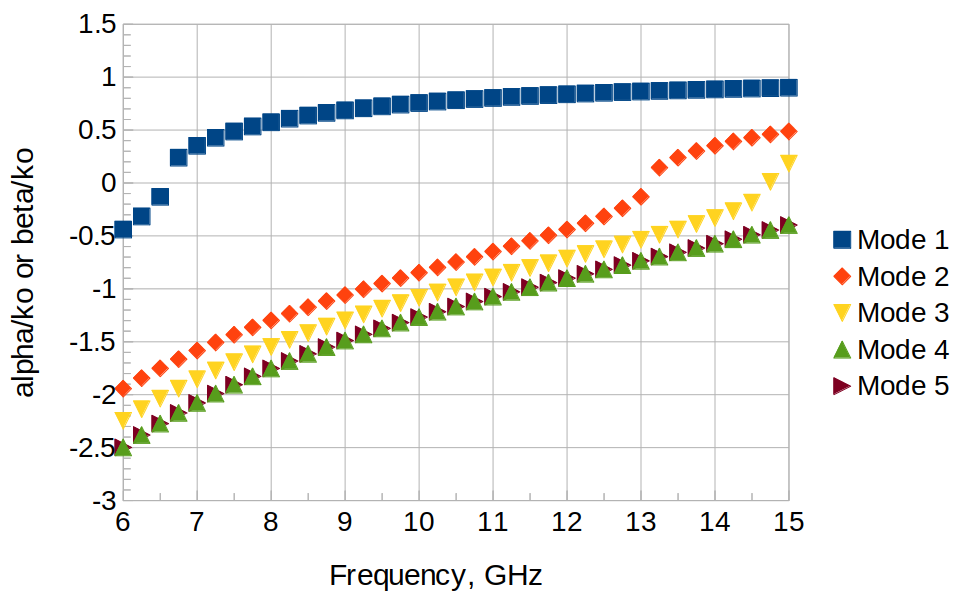
\includegraphics[width=0.5\textwidth]{../regression/OpenParEM2D/WR90_rectangular_waveguide/WR90/WR90_order_6_study/screenshots/WR90_gamma}
  \caption{$\gamma$ for the first 5 modes of the lossless WR90 rectangular waveguide.}
  \label{fig:WR90_gamma}
\end{figure}

\begin{figure}[H]
  \centering
  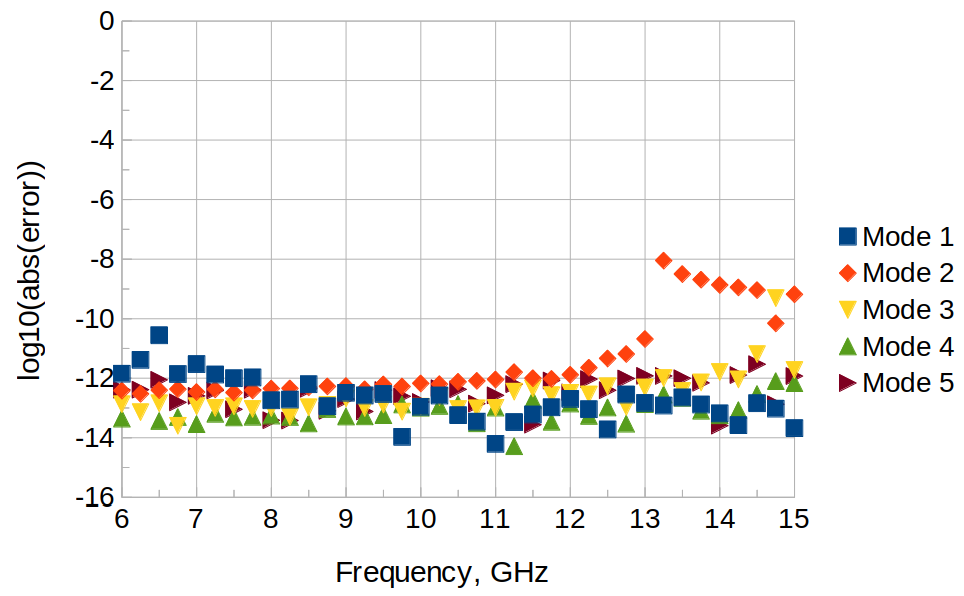
\includegraphics[width=0.5\textwidth]{../regression/OpenParEM2D/WR90_rectangular_waveguide/WR90/WR90_order_6_study/screenshots/WR90_gamma_error}
  \caption{Error in $\gamma$ for the first 5 modes of the lossless WR90 rectangular waveguide.}
  \label{fig:WR90_gamma_error}
\end{figure}

The characteristic impedance and the error vs. the theoretical result for the dominant mode is shown in Fig.~\ref{fig:WR90_impedance}.  The baseline error is about $10^{-9}$.

\begin{figure}[H]
  \centering
  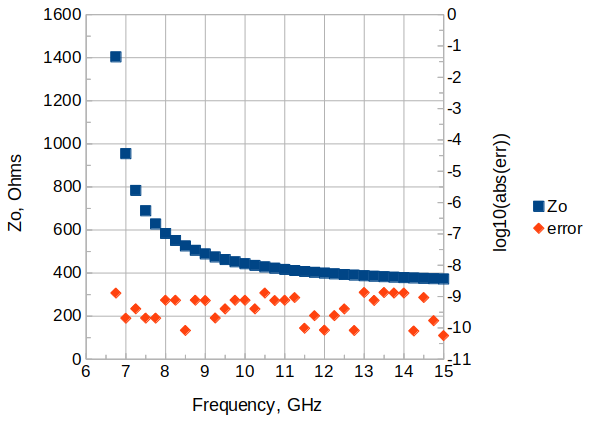
\includegraphics[width=0.5\textwidth]{../regression/OpenParEM2D/WR90_rectangular_waveguide/WR90/WR90_order_6_study/screenshots/WR90_impedance}
  \caption{Impedance and error for the dominant mode of the lossless WR90 rectangular waveguide.}
  \label{fig:WR90_impedance}
\end{figure}

A field plot for the dominant mode at 10~GHz is shown in Fig.~\ref{fig:WR90_mode_1}, where the black arrows show $\textnormal{Re}(\overline{E})$, the white arrows show $\textnormal{Re}(\overline{H})$, and the background shows $\textnormal{Re}(|\overline{E}|)$.  Note that $\textnormal{Re}(\overline{E})$ and $\textnormal{Re}(\overline{H})$ are plotted with different scales.
\begin{figure}[H]
  \centering
  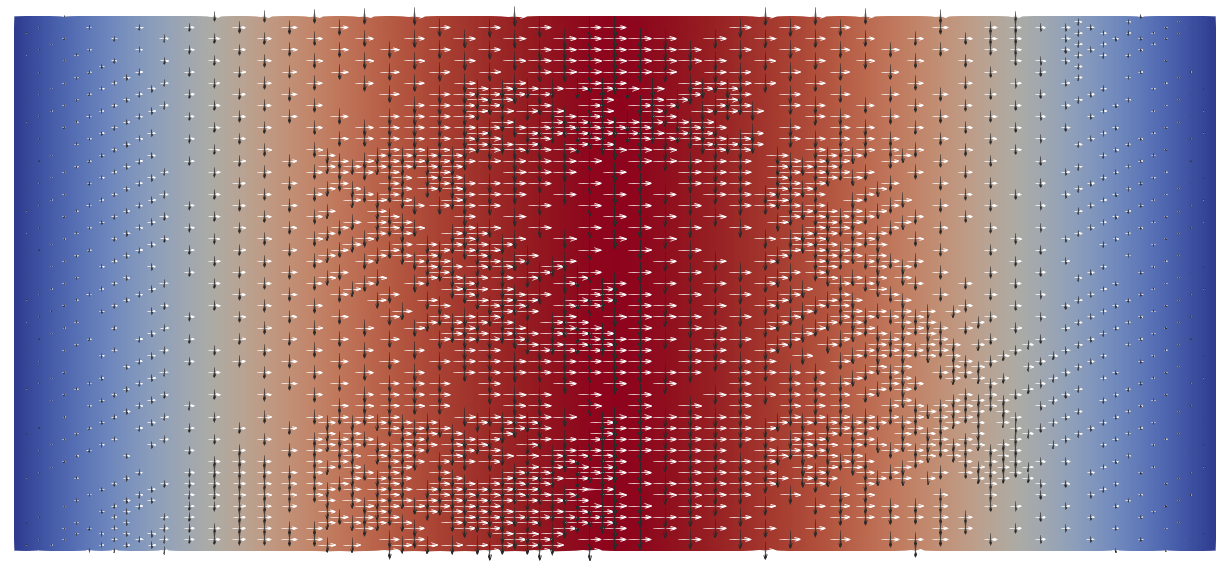
\includegraphics[width=0.66\textwidth]{../regression/OpenParEM2D/WR90_rectangular_waveguide/WR90/WR90_order_6_study/screenshots/WR90_mode_1}
  \caption{Field plot for the dominant mode of the lossless WR90 rectangular waveguide.}
  \label{fig:WR90_mode_1}
\end{figure}
An interesting but not very useful plot of the real power flow in the longitudinal direction of the cutoff 4$^{\textnormal{th}}$ mode is shown in Fig.~\ref{fig:WR90_mode_4_Pz}, showing that real power flows in both directions but must balance to zero since the mode is cut off.
\begin{figure}[H]
  \centering
  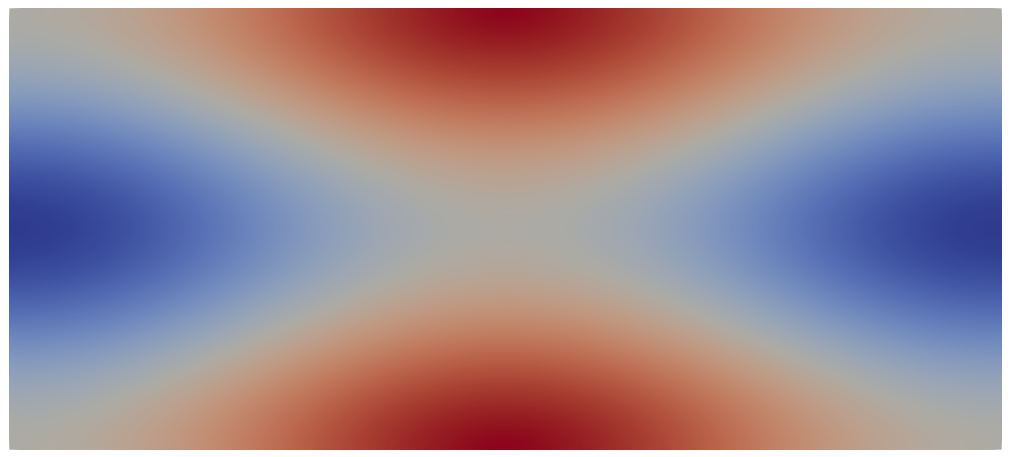
\includegraphics[width=0.65\textwidth]{../regression/OpenParEM2D/WR90_rectangular_waveguide/WR90/WR90_order_6_study/screenshots/WR90_mode_4_Pz}
  \caption{Longitudinal power flow for the 4$^{\textnormal{th}}$ mode of the lossless WR90 rectangular waveguide.}
  \label{fig:WR90_mode_4_Pz}
\end{figure}

\subsection{Lossy WR90 Waveguide}

The lossless WR90 waveguide of Sec.~\ref{sec:WR90_lossless} is re-simulated for the dominant mode including finite conductivity on the walls of the waveguide.  OpenParEM2D first simulates the lossless case then uses the computed fields to calculate the losses on the conductive boundaries and adds those losses to the dielectric losses directly computed as part of the eigenvalue problem solution.  For this case, there are no dielectric losses, so all of the losses are due to the losses on the finite-conductivity boundary.

The lossy WR90 rectangular waveguide project can be found in the OpenParEM2D distribution in \texttt{regression/WR90\_rectangular\_waveguide/WR90/WR90\_order\_6\_lossy\_study}. The solution uses 6$^{\textnormal{th}}$-order finite elements. The mesh is optimized at 11~GHz starting with a very sparse mesh of just 4 elements that is then uniformly refined once then adaptively refined. The optimization variable is $\alpha$ with a relative tolerance of $10^{-10}$ with two consecutive iterations and a solution tolerance of $10^{-13}$. After optimization at 11~GHz, the frequency is swept from 6.75~GHz to 15~GHz.

The propagation constant $\gamma$ is shown in Fig.~\ref{fig:WR90_lossy_gamma}.  The theoretical result is provided by \cite{Ramo} in (17) on p.~417, and the error vs. the theoretical result is shown in Fig.~\ref{fig:WR90_lossy_gamma_error}.  At the mesh optimization frequency of 11~GHz, the error for $\alpha/k_{\circ}$ is about $10^{-10}$ and about $10^{-12}$ for $\beta/k_{\circ}$.  Over the entire sweep, the worst-case error for $\alpha/k_{\circ}$ drops about 1 order of magnitude, while for $\beta/k_{\circ}$ it drops less than 2 orders of magnitude as frequency decreases, so the error is still excellent over this 2:1 frequency span with a mesh optimized at a center frequency.

\begin{figure}[H]
  \centering
  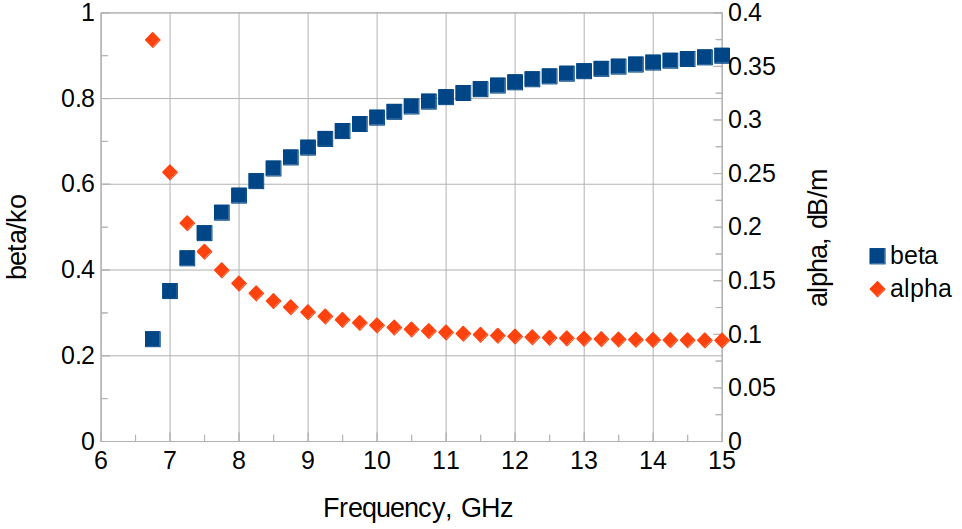
\includegraphics[width=0.55\textwidth]{../regression/OpenParEM2D/WR90_rectangular_waveguide/WR90/WR90_order_6_lossy_study/screenshots/WR90_lossy_gamma}
  \caption{$\gamma$ for the dominant mode of the lossy WR90 rectangular waveguide.}
  \label{fig:WR90_lossy_gamma}
\end{figure}

\begin{figure}[H]
  \centering
  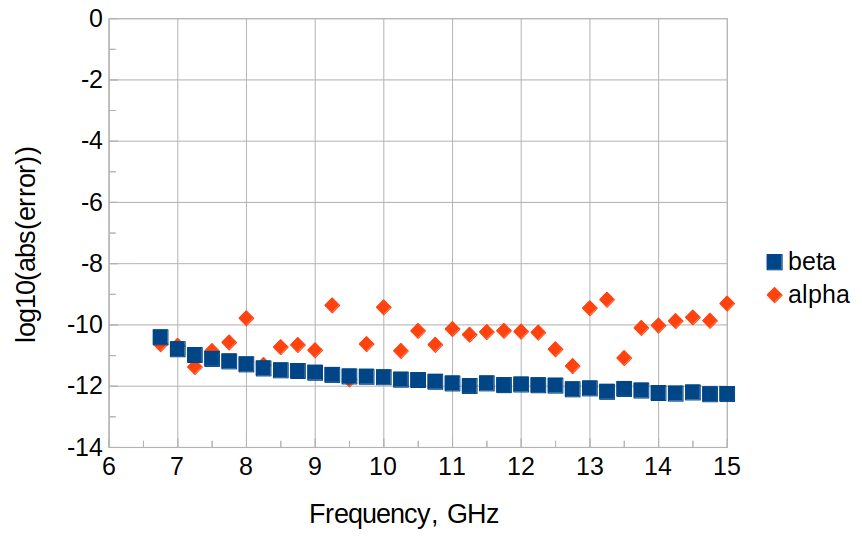
\includegraphics[width=0.5\textwidth]{../regression/OpenParEM2D/WR90_rectangular_waveguide/WR90/WR90_order_6_lossy_study/screenshots/WR90_lossy_gamma_error}
  \caption{Error in $\gamma$ for the dominant mode of the lossy WR90 rectangular waveguide.}
  \label{fig:WR90_lossy_gamma_error}
\end{figure}

\subsection{Partially-Filled Rectangular Waveguide}

A lossless partially-filled rectangular waveguide is simulated for comparison against numerical solution of the transcendental equation of the exact result. The project can be found in the OpenParEM2D distribution in \texttt{regression/partially\_filled\_rect\_waveguide/PartFilled\_order\_6\_study}.  The studied example is taken from \cite{Harrington}, Fig.~4.7 on p.~161.  The waveguide is shown in Fig.~\ref{fig:partial_drawing}.
\begin{figure}[H]
  \centering
  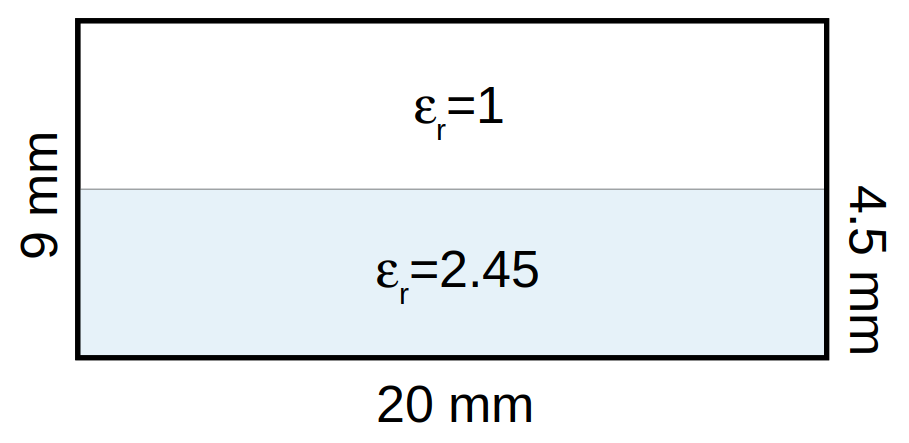
\includegraphics[width=0.3\textwidth]{../regression/OpenParEM2D/partially_filled_rect_waveguide/PartFilled_order_6_study/screenshots/partial_drawing}
  \caption{A partially-filled waveguide for analysis.}
  \label{fig:partial_drawing}
\end{figure}

The transcendental equation providing the complex propagation constant is given in \cite{Harrington} equations (4-56) and (4-58).  These are solved in \texttt{waveguide.c} in the OpenParEM2D source directory.

The propagation constant $\gamma$ is shown in Fig.~\ref{fig:partial_gamma}, where $\gamma$ is plotted as either $\alpha/k_{\circ}$ when a mode is cut off or $\beta/k_{\circ}$ when it is propagating.  The error vs. the transcendental solution of the exact theoretical result is shown in Fig.~\ref{fig:partial_gamma_error}, where the baseline error is about $10^{-12}$ except for the expected increase as $\gamma$ transitions through zero.

\begin{figure}[H]
  \centering
  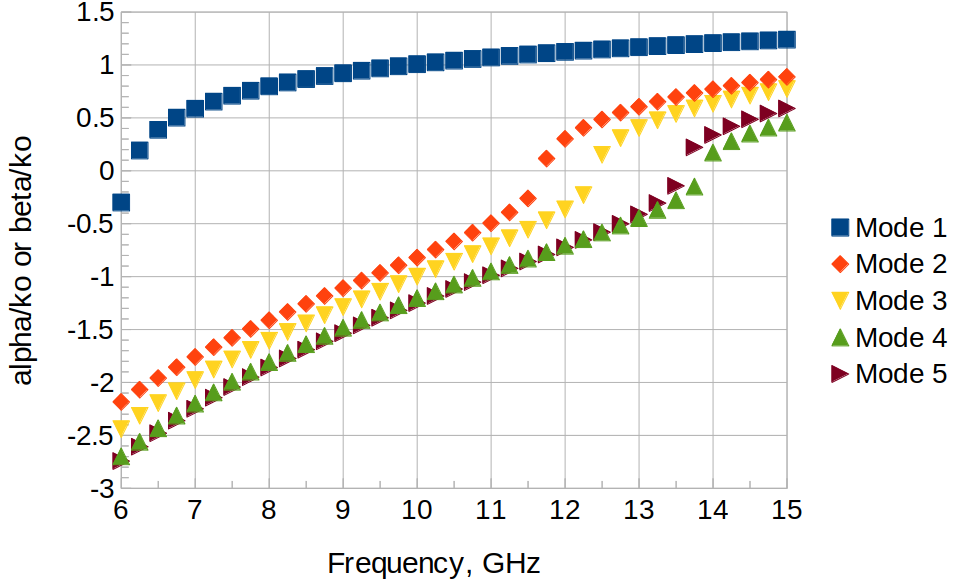
\includegraphics[width=0.5\textwidth]{../regression/OpenParEM2D/partially_filled_rect_waveguide/PartFilled_order_6_study/screenshots/partial_gamma}
  \caption{$\gamma$ for the first 5 modes of the partially filled rectangular waveguide.}
  \label{fig:partial_gamma}
\end{figure}

\begin{figure}[H]
  \centering
  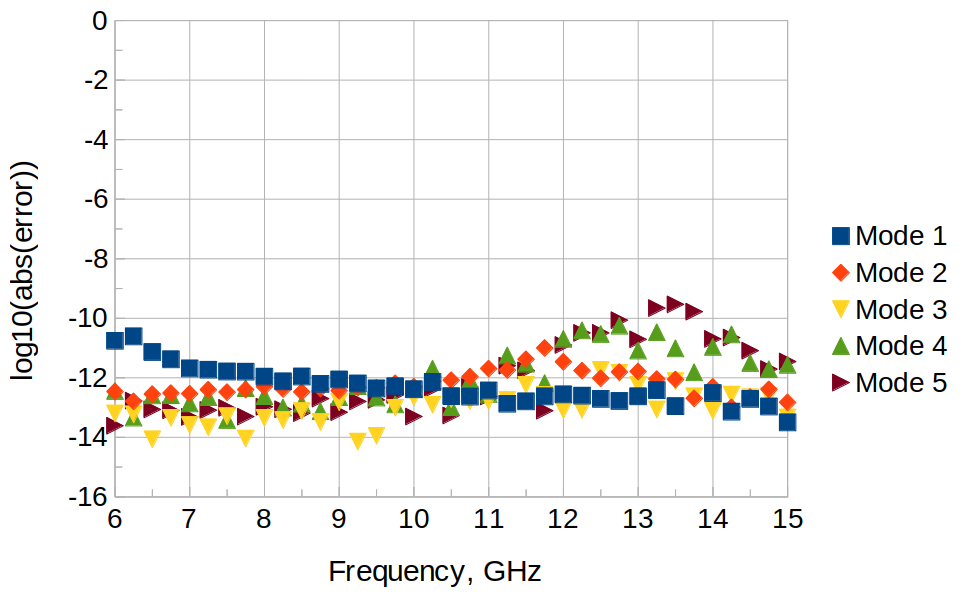
\includegraphics[width=0.5\textwidth]{../regression/OpenParEM2D/partially_filled_rect_waveguide/PartFilled_order_6_study/screenshots/partial_gamma_error}
  \caption{Error in $\gamma$ for the first 5 modes of the partially filled rectangular waveguide.}
  \label{fig:partial_gamma_error}
\end{figure}

Plots of the dominant mode at 10~GHz are shown in Fig.~\ref{fig:partial_field_power}. The fields plot uses black arrows for $\textnormal{Re}(\overline{E})$, white arrows for $\textnormal{Re}(\overline{H})$, and the background shows $\textnormal{Re}(|\overline{E}|)$. Note that $\textnormal{Re}(\overline{E})$ and $\textnormal{Re}(\overline{H})$ use different scales. The power plot shows the longitudinal component of the real part of the Poynting vector, and since this mode is propagating, the power is always positive. 

\begin{figure}[H]
  \centering
  \begin{subfigure}{0.429\textwidth}
     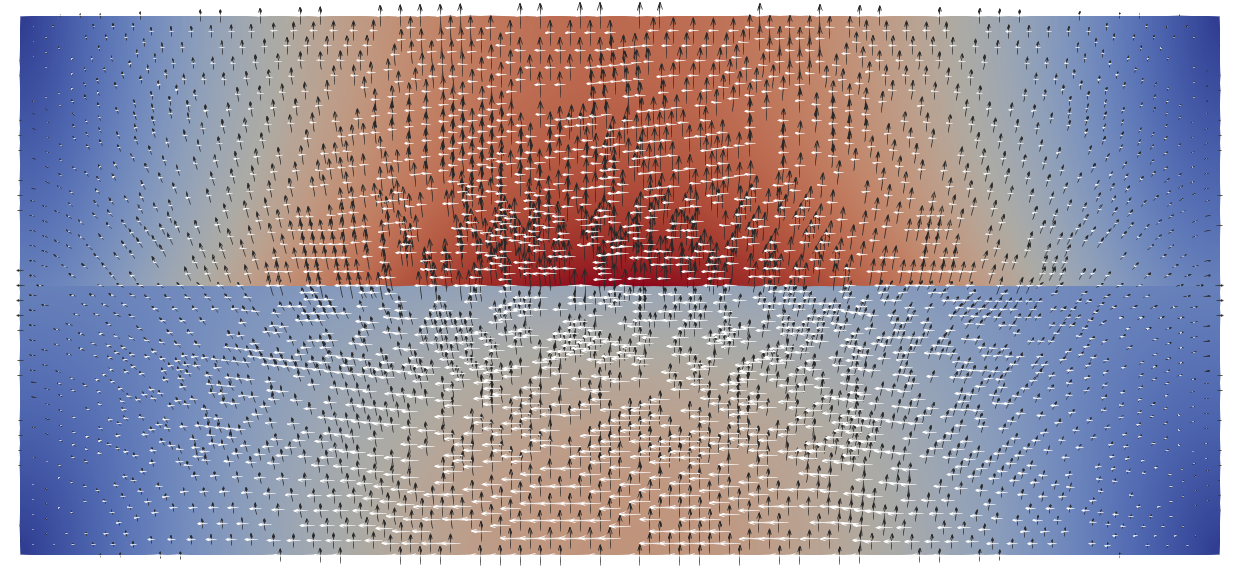
\includegraphics[width=\linewidth]{../regression/OpenParEM2D/partially_filled_rect_waveguide/PartFilled_order_6_study/screenshots/partial_field}
     \caption{Fields.}
  \end{subfigure}
  \begin{subfigure}{0.471\textwidth}
     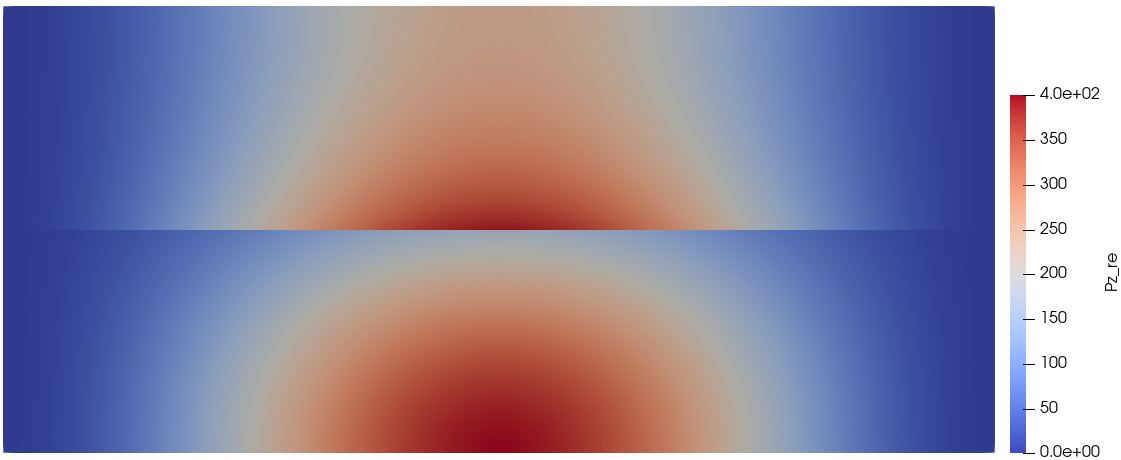
\includegraphics[width=\linewidth]{../regression/OpenParEM2D/partially_filled_rect_waveguide/PartFilled_order_6_study/screenshots/partial_power}
     \caption{Power in longitudinal direction.}
  \end{subfigure}
  \caption{Computed solutions for the dominant mode at 10 GHz.}
  \label{fig:partial_field_power}
\end{figure}

\subsection{Coaxial Waveguide}

A lossless coaxial waveguide is simulated for comparison against exact results.  The project can be found in the OpenParEM2D distribution in \texttt{regression/coaxEighth\_study}.  The coax has an inner conductor radius of 0.406~mm, an outer radius of 1.48~mm, and a dielectric with $\epsilon_r=2.26$.  The structure is drawn in FreeCAD using polygons with 10 segments per 45$^{\circ}$. Using symmetry with PMC boundaries, 1/8 of the structure is simulated.  Assuming perfect circles, the exact impedance is 51.5874640385028~$\Omega$.  Since this is a lossless TEM transmission line, the exact value for $\beta/k_{\circ}=\sqrt{2.26}$.

The simulation uses 2$^{\textnormal{nd}}$-order finite elements with adaptive refinement stepping down in frequency from 10,000~GHz to 10~MHz in 10$\times$ steps to avoid potential convergence issues at low frequencies.  Since the mesh is refined multiple times, the relative tolerance is set to a somewhat loose value of $10^{-5}$ converging on $|Z_{\circ}|$.

A field plot is shown in Fig.~\ref{fig:coax_field}, where black arrows show $\textnormal{Re}(\overline{E})$, white arrows $\textnormal{Re}(\overline{H})$, and the background shows $\textnormal{Re}(|\overline{E}|)$.  Note that $\textnormal{Re}(\overline{E})$ and $\textnormal{Re}(\overline{H})$ use different scales. The real power traveling down the coax is shown in Fig.~\ref{fig:coax_Pz}, where the power concentrates near the center conductor.

\begin{figure}[H]
  \centering
  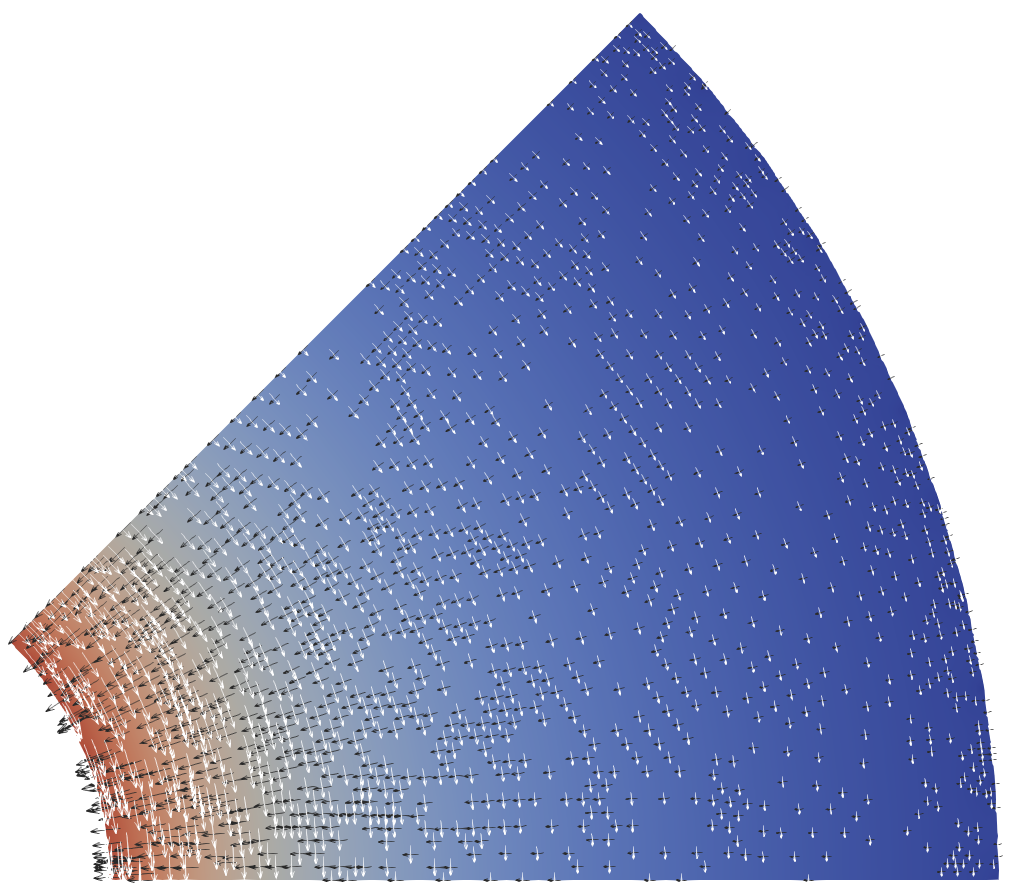
\includegraphics[width=0.5\textwidth]{../regression/OpenParEM2D/coaxEighth_study/screenshots/coax_field}
  \caption{Field plot for the coaxial waveguide at 1 GHz.}
  \label{fig:coax_field}
\end{figure}

\begin{figure}[H]
  \centering
  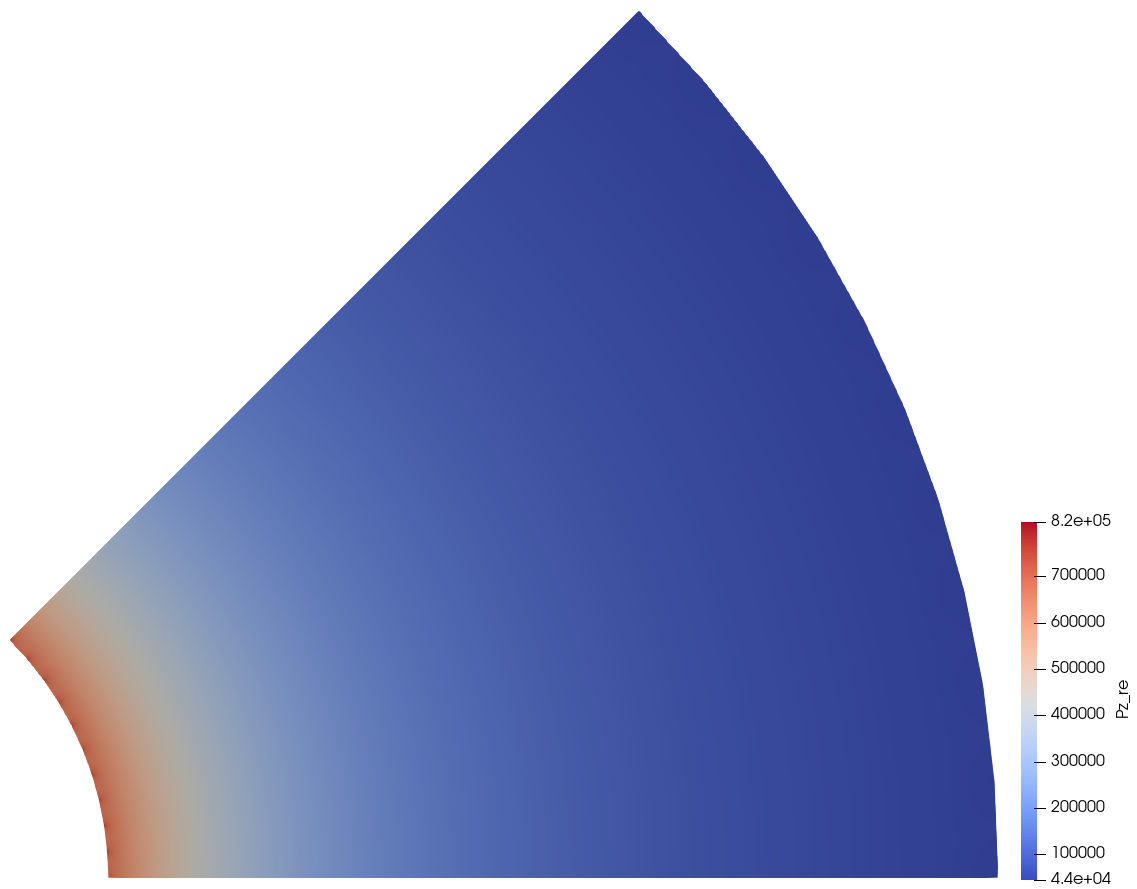
\includegraphics[width=0.53\textwidth]{../regression/OpenParEM2D/coaxEighth_study/screenshots/coax_Pz}
  \caption{Real power flow for the coaxial waveguide at 1 GHz.}
  \label{fig:coax_Pz}
\end{figure}

The results are plotted as errors vs. the exact values in Fig.~\ref{fig:coax_results}. The error for $\beta/k_{\circ}$ steadily reduces with increasing frequency until numerical precision is reached around $10^{-14}$.  Note that an exact match is achieved at two frequencies.  As frequency decreases, the error for $\beta/k_{\circ}$ steadily increases until the error fails to meet engineering-level precision of 1\% [-2 on the log scale] at about 1~MHz.  The reduction in accuracy is due to Faraday's and Ampere's laws progressively decoupling requiring more numerical precision than double-precision calculations can provide.  The error for $Z_{\circ}$ behaves in a similar fashion to $\beta/k_{\circ}$ except that the error plateaus at -4.7 [on a log scale] due to the circular structure being modeled as polygons. A zoom of the power real flow near the conductor is shown in Fig.~\ref{fig:coax_Pz_zoom}, where the points on the polygon approximation causes local increases in power, leading to a small increase in the overall power flow with a consequent small reduction in $Z_{\circ}$, so a small increase in the error, since power appears in the denominator in the power-voltage definition of $Z_{\circ}$.
\begin{figure}[H]
  \centering
  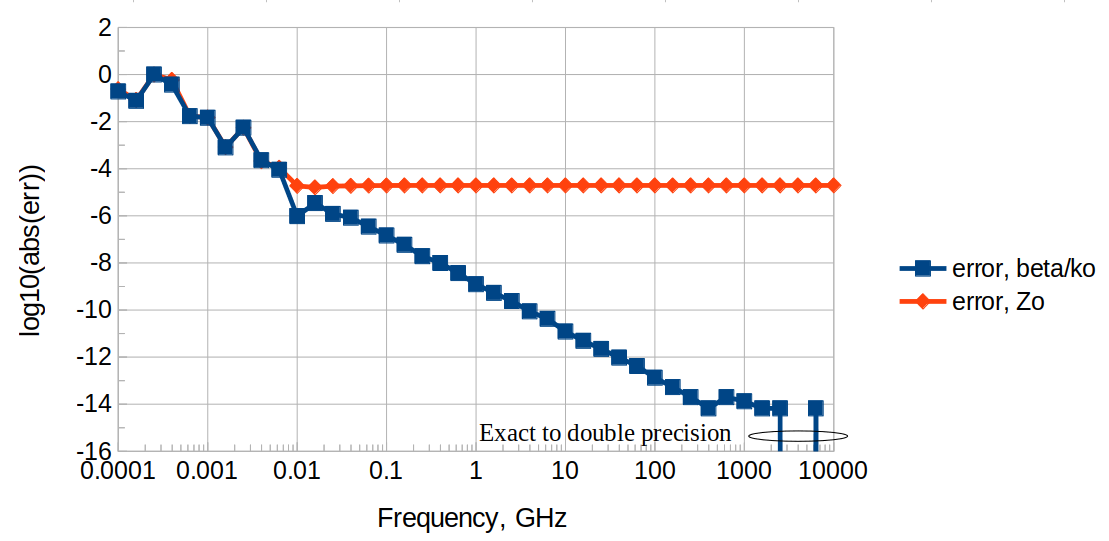
\includegraphics[width=0.65\textwidth]{../regression/OpenParEM2D/coaxEighth_study/screenshots/coax_results}
  \caption{Error vs. exact values for the coaxial waveguide.}
  \label{fig:coax_results}
\end{figure}
\begin{figure}[H]
  \centering
  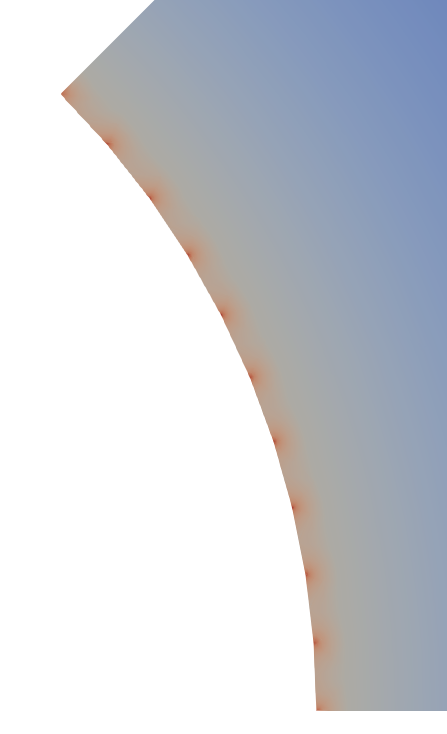
\includegraphics[width=0.25\textwidth]{../regression/OpenParEM2D/coaxEighth_study/screenshots/coax_Pz_zoom}
  \caption{Zoom with re scale of the power flow from Fig.~\ref{fig:coax_Pz} near the center conductor.}
  \label{fig:coax_Pz_zoom}
\end{figure}

\subsection{Coupled Microstrip}

A coupled microstrip is simulated and compared to the simulations for the case in Fig.~8 from \cite{Olyslager}.  The project can be found in the OpenParEM2D distribution in \texttt{regression/differential\_pair/diff\_pair\_study}.  The structure is drawn and set up in FreeCAD, meshed with gmsh \cite{gmsh}\cite{gmshweb}, then solved using 3$^{\textnormal{rd}}$-order finite elements with adaptive refinement sequencing from 100~GHz to 52~GHz to 8~GHz with a relative tolerance of 0.001 optimizing on $|Z_{\circ}|$.

The initial mesh produced by gmsh is shown in Fig.~\ref{fig:diffpair_initial_mesh}.  After adaptive mesh refinement, the final mesh is shown in Fig.~\ref{fig:diffpair_optimized_mesh}, where the adaptive mesh refinement algorithm has concentrated mesh refinement in areas of rapid changes in the fields near the corners of the strips.
\begin{figure}[H]
  \centering
  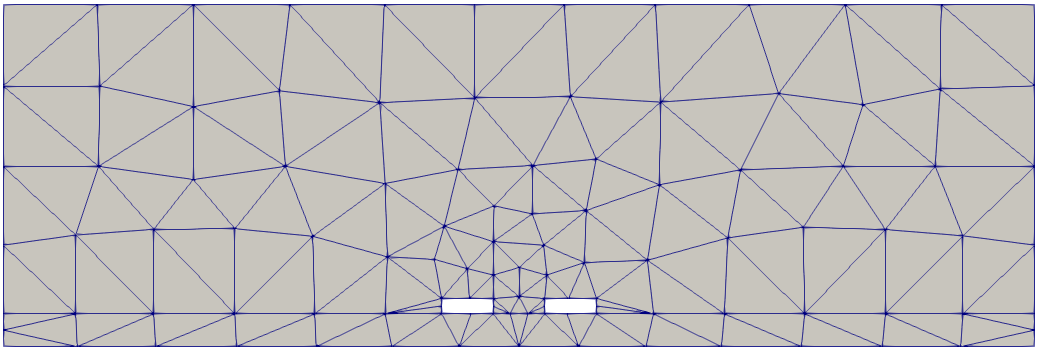
\includegraphics[width=0.5\textwidth]{../regression/OpenParEM2D/differential_pair/diff_pair_study/screenshots/diffpair_initial_mesh}
  \caption{Initial mesh before adaptive refinement.}
  \label{fig:diffpair_initial_mesh}
\end{figure}
\begin{figure}[H]
  \centering
  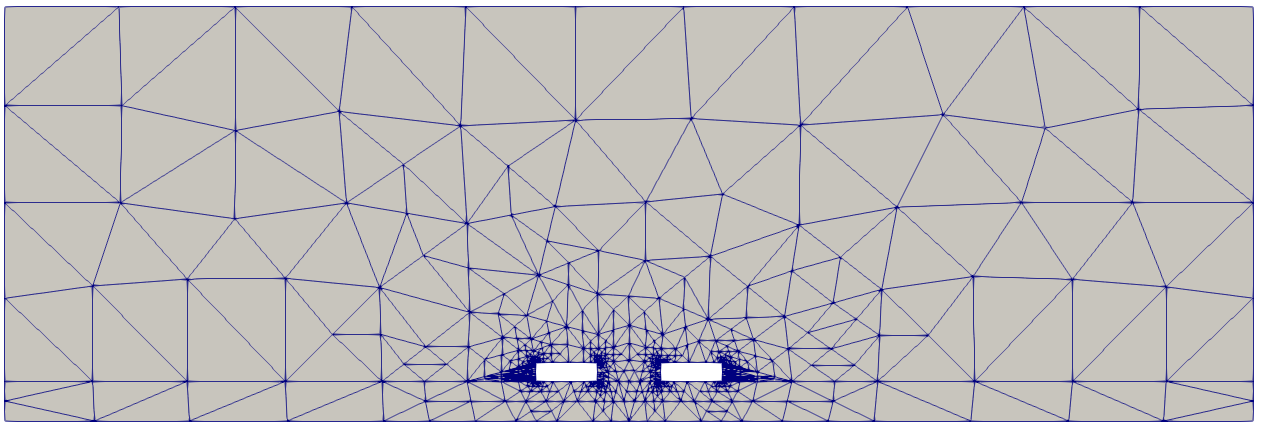
\includegraphics[width=0.5\textwidth]{../regression/OpenParEM2D/differential_pair/diff_pair_study/screenshots/diffpair_optimized_mesh}
  \caption{Final mesh after adaptive refinement.}
  \label{fig:diffpair_optimized_mesh}
\end{figure}

Results are compared with those scaled off the plots from \cite{Olyslager} in Fig.~\ref{fig:diffpair_even} for the even mode and Fig.~\ref{fig:diffpair_odd} for the odd mode.  For both modes, agreement is excellent for the propagation constant and good for the characteristic impedance.
\begin{figure}[H]
  \centering
  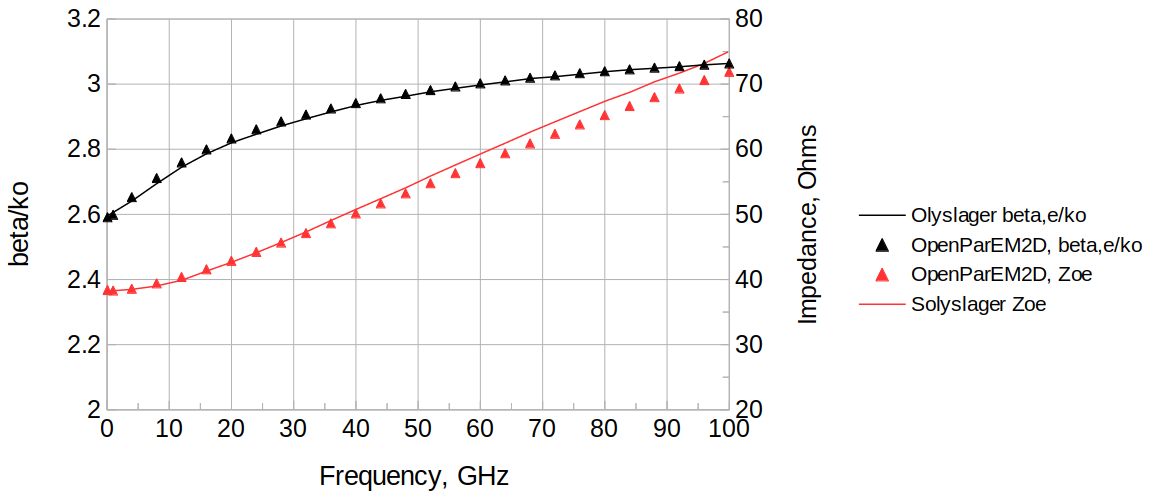
\includegraphics[width=0.7\textwidth]{../regression/OpenParEM2D/differential_pair/diff_pair_study/screenshots/diffpair_even}
  \caption{Even mode results for the coupled microstrip from Fig. 8 in \cite{Olyslager}.}
  \label{fig:diffpair_even}
\end{figure}
\begin{figure}[H]
  \centering
  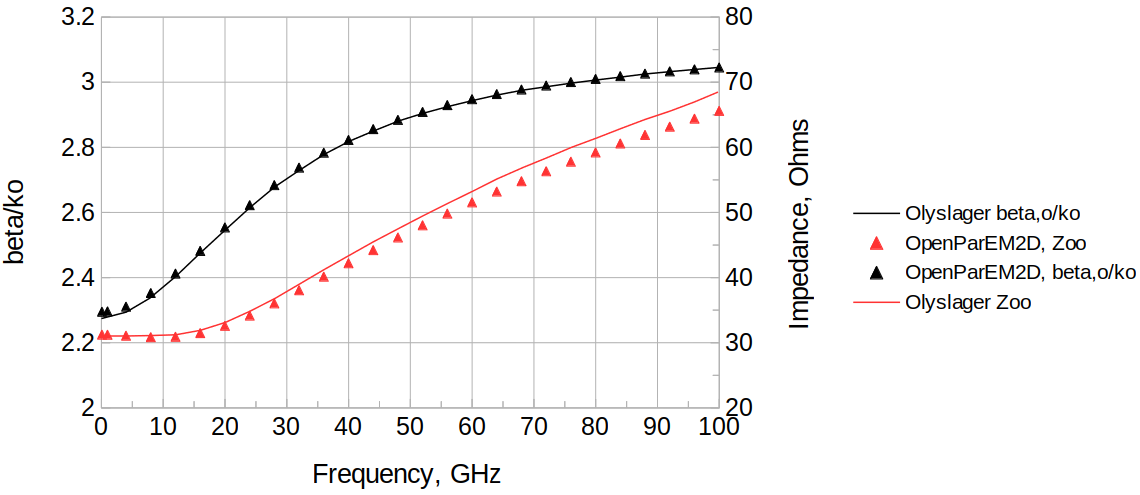
\includegraphics[width=0.7\textwidth]{../regression/OpenParEM2D/differential_pair/diff_pair_study/screenshots/diffpair_odd}
  \caption{odd mode results for the coupled microstrip from Fig. 8 in \cite{Olyslager}.}
  \label{fig:diffpair_odd}
\end{figure}

Plots of the fields at 52~GHz are shown in Fig.~\ref{fig:diffpair_even_plot} for the even mode and Fig.~\ref{fig:diffpair_odd_plot} for the odd mode, where black arrows show $\textnormal{Re}(\overline{E})$, white arrows $\textnormal{Re}(\overline{H})$, and the background shows $\textnormal{Re}(|\overline{E}|)$ with 16 levels of discretization to show the iso field lines.  Note that $\textnormal{Re}(\overline{E})$ and $\textnormal{Re}(\overline{H})$ use different scales.
\begin{figure}[H]
  \centering
  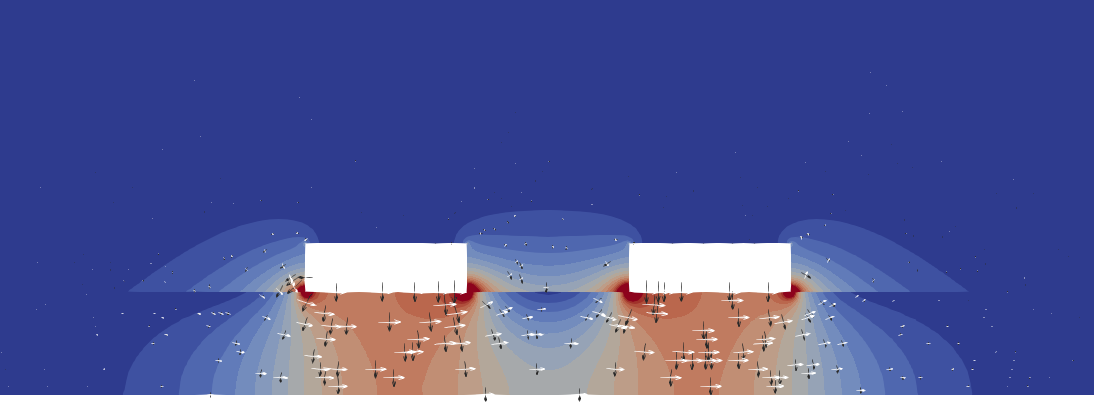
\includegraphics[width=0.65\textwidth]{../regression/OpenParEM2D/differential_pair/diff_pair_study/screenshots/diffpair_even_plot}
  \caption{Plot of the even mode fields.}
  \label{fig:diffpair_even_plot}
\end{figure}
\begin{figure}[H]
  \centering
  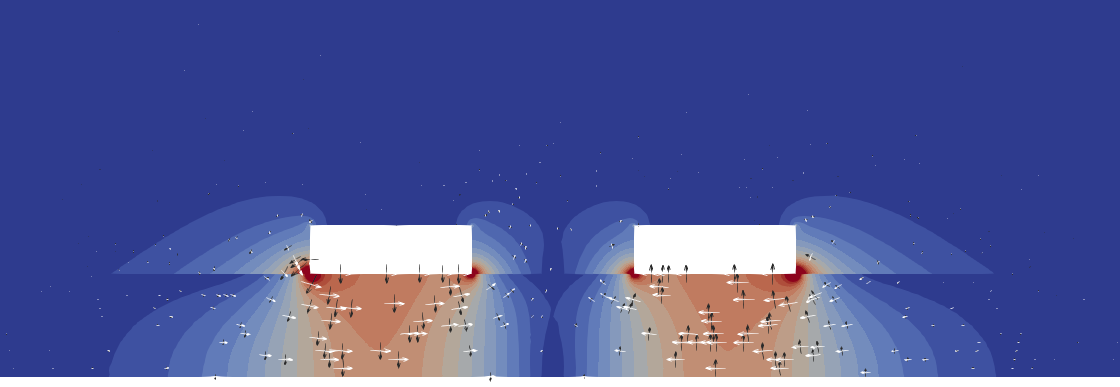
\includegraphics[width=0.65\textwidth]{../regression/OpenParEM2D/differential_pair/diff_pair_study/screenshots/diffpair_odd_plot}
  \caption{Plot of the odd mode fields.}
  \label{fig:diffpair_odd_plot}
\end{figure}

\subsection{Lossy Stripline}

A lossy stripline is simulated and compared to the simulations and measurements from the case in Fig.~16, right-hand graph, from \cite{Simonovich}.  The project can be found in the OpenParEM2D distribution in \texttt{regression/Simonovich\_stripline\_study}.  The structure is set up using \texttt{builder}, meshed with gmsh, then solved using 2$^{\textnormal{nd}}$-order finite elements with adaptive refinement at 50~GHz optimizing on alpha.  This case demonstrates the accuracy of the surface roughness modeling.

The initial mesh in Fig.~\ref{fig:stripline_initial_mesh} is fairly dense with extensive mesh away from the strip.  This makes the problem susceptible to over-meshing.  Since the bulk of the needed mesh refinement is near the corners of the trace, a low value of 0.01 is set for \texttt{mesh.refinement.fraction} so that a relatively small number of elements are refined at each pass, minimizing the number of elements refined away from the trace. Second order elements also help minimize issues with over-meshing with the large number of elements far from the trace having virtually no field variation.  Two signs of over-meshing that can appear with this simulation are failure to converge with a tight convergence tolerance and failure of convergence for $\overline{H}$ without setting a much smaller value for \texttt{solution.tolerance}, such as $10^{-8}$. The final mesh is shown in Fig.~\ref{fig:stripline_final_mesh} along with zooms in Figs.~\ref{fig:stripline_mesh_zoom1} and \ref{fig:stripline_mesh_zoom2}.

\begin{figure}[H]
  \centering
  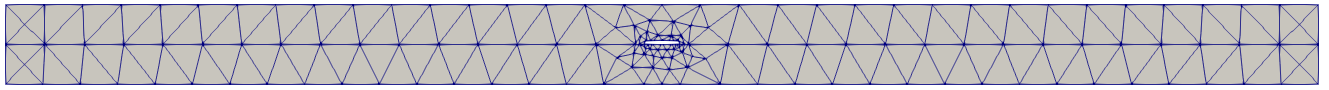
\includegraphics[width=0.95\textwidth]{../regression/OpenParEM2D/Simonovich_stripline_study/screenshots/stripline_initial_mesh}
  \caption{Initial mesh.}
  \label{fig:stripline_initial_mesh}
\end{figure}
\begin{figure}[H]
  \centering
  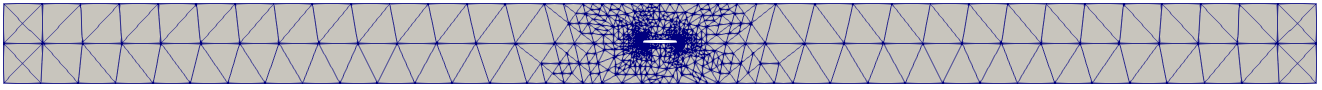
\includegraphics[width=0.95\textwidth]{../regression/OpenParEM2D/Simonovich_stripline_study/screenshots/stripline_final_mesh}
  \caption{Final optimized mesh.}
  \label{fig:stripline_final_mesh}
\end{figure}
\begin{figure}[H]
  \centering
  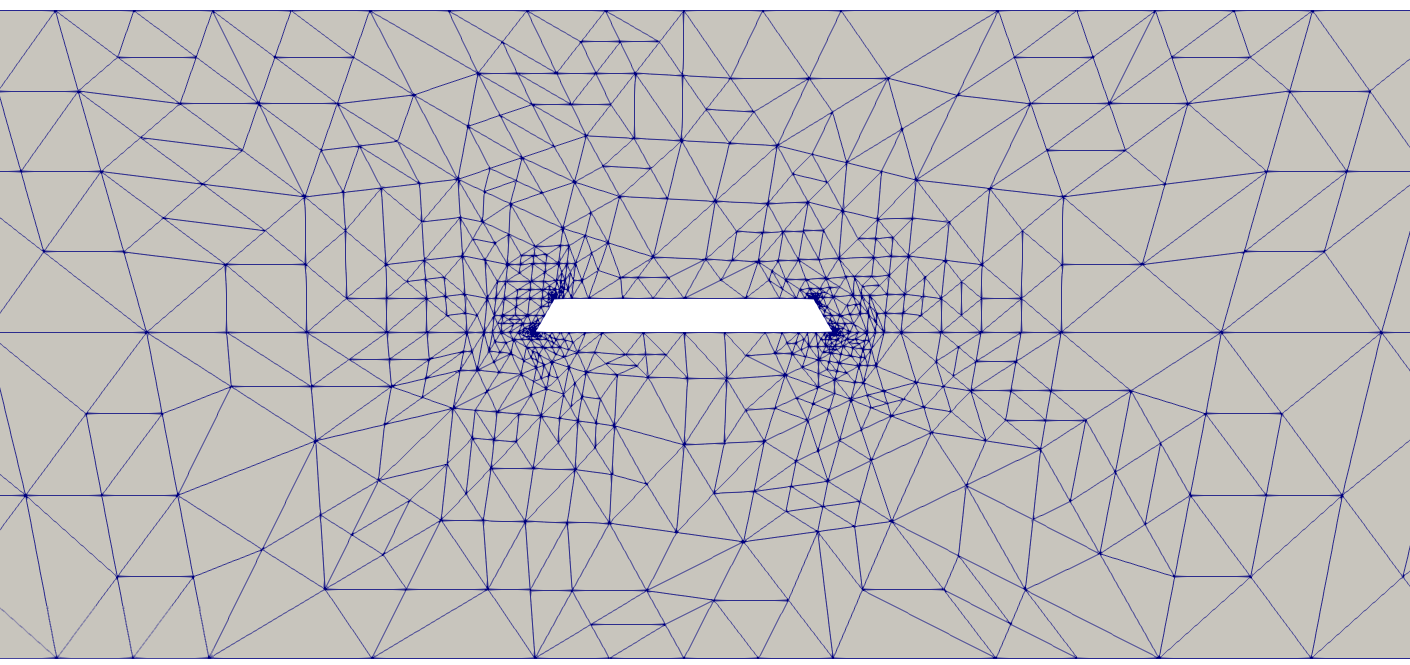
\includegraphics[width=0.6\textwidth]{../regression/OpenParEM2D/Simonovich_stripline_study/screenshots/stripline_mesh_zoom1}
  \caption{Zoom of the final optimized mesh around the trace.}
  \label{fig:stripline_mesh_zoom1}
\end{figure}
\begin{figure}[H]
  \centering
  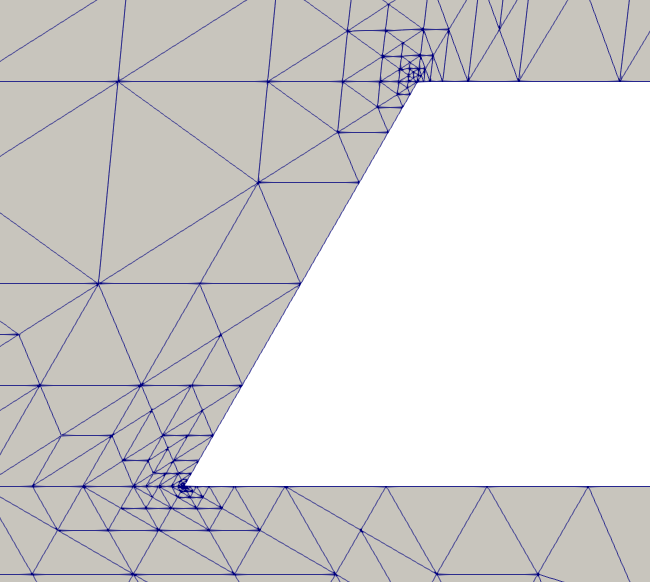
\includegraphics[width=0.5\textwidth]{../regression/OpenParEM2D/Simonovich_stripline_study/screenshots/stripline_mesh_zoom2}
  \caption{Zoom of the final optimized mesh around the left side trace corners.}
  \label{fig:stripline_mesh_zoom2}
\end{figure}

Results are compared with those scaled off the plot in \cite{Simonovich} in Fig.~\ref{fig:stripline_results}, where the results are in very good agreement.  Errors are plotted in Fig.~\ref{fig:stripline_error}. A field plot at 50 GHz is shown in Fig.~\ref{fig:stripline_plot}, where black arrows show $\textnormal{Re}(\overline{E})$, white arrows $\textnormal{Re}(\overline{H})$, and the background shows $\textnormal{Re}(|\overline{E}|)$ with 32 levels of discretization to show the iso field lines. Note that $\textnormal{Re}(\overline{E})$ and $\textnormal{Re}(\overline{H})$ use different scales.
\begin{figure}[H]
  \centering
  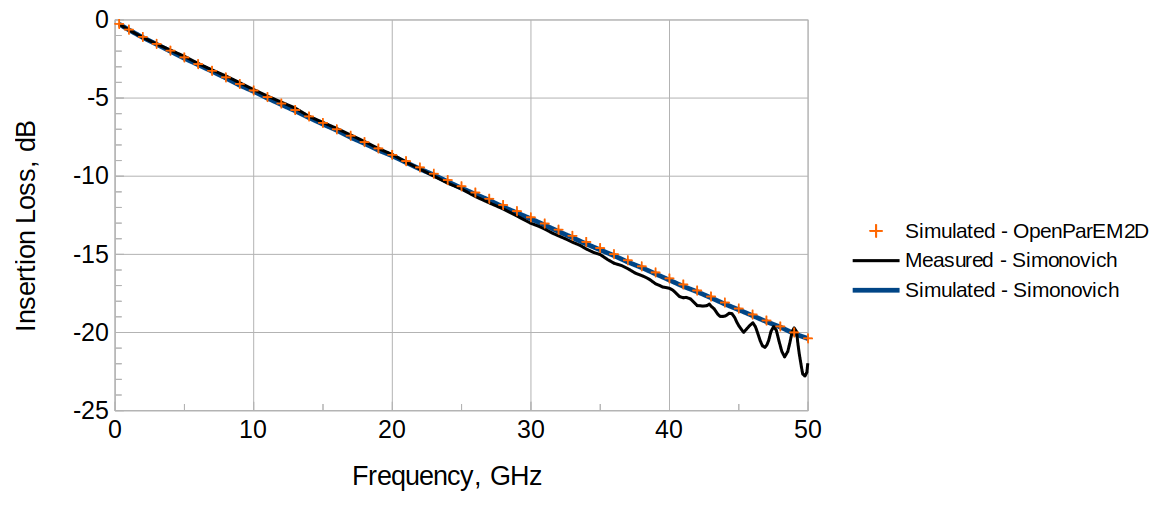
\includegraphics[width=0.75\textwidth]{../regression/OpenParEM2D/Simonovich_stripline_study/screenshots/stripline_results}
  \caption{Attenuation results for the case from Fig. 16 in \cite{Simonovich}.}
  \label{fig:stripline_results}
\end{figure}
\begin{figure}[H]
  \centering
  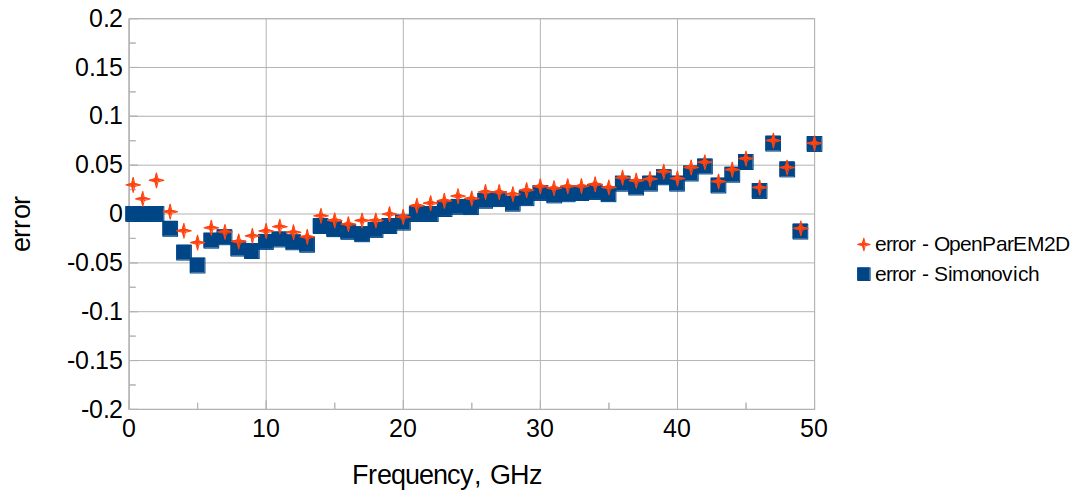
\includegraphics[width=0.75\textwidth]{../regression/OpenParEM2D/Simonovich_stripline_study/screenshots/stripline_error}
  \caption{Error plot for attenuation.}
  \label{fig:stripline_error}
\end{figure}
\begin{figure}[H]
  \centering
  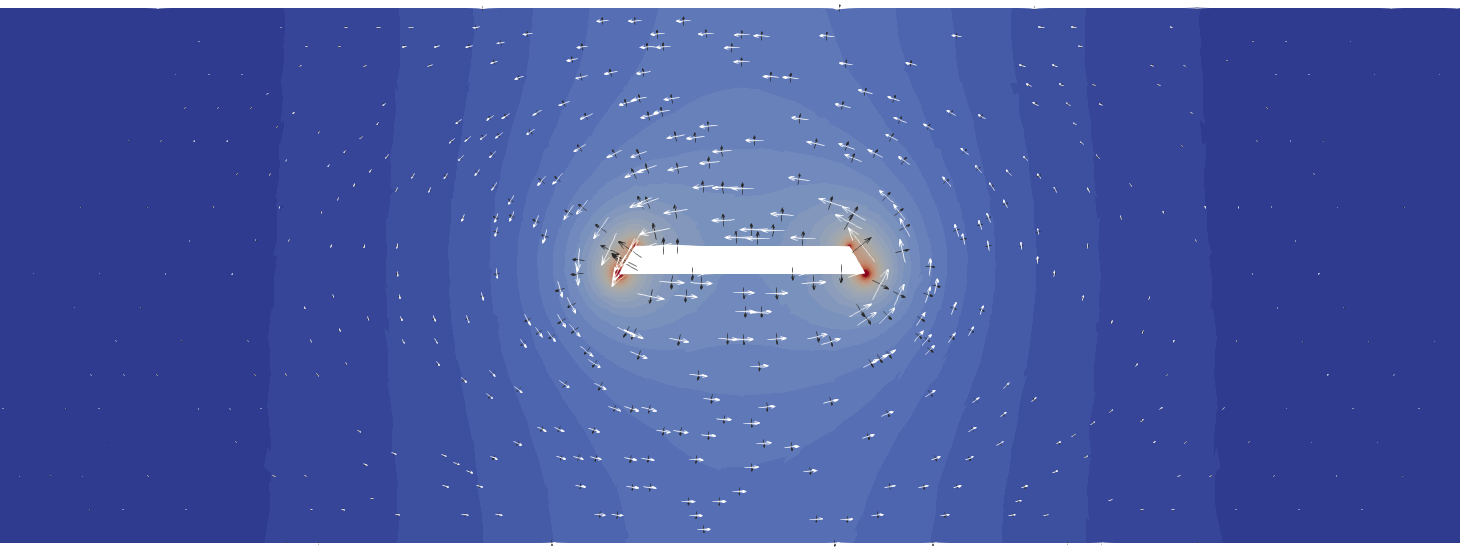
\includegraphics[width=0.75\textwidth]{../regression/OpenParEM2D/Simonovich_stripline_study/screenshots/stripline_plot}
  \caption{Field plot at 50 GHz.}
  \label{fig:stripline_plot}
\end{figure}





\begin{thebibliography}{unsrt}

\bibitem{MFEM} R. Anderson, J. Andrej, A. Barker, J. Bramwell, J.-S. Camier, J. Cerveny, V. Dobrev, Y. Dudouit, A. Fisher, Tz. Kolev, W. Pazner, M. Stowell, V. Tomov, I. Akkerman, J. Dahm, D. Medina, and S. Zampini, "MFEM: A modular finite element methods library", \textit{Computers and Mathematics with Applications}, vol. 81, 2021, pp. 42-74.

\bibitem{MFEMweb} \verb+https://mfem.org+

\bibitem{Lee} Jin-Fa Lee, “Finite element analysis of lossy dielectric waveguides”, \textit{IEEE Tran. Microwave Theory and Techniques}, vol. 42, no. 6, June 1994, pp. 1025-1031.

\bibitem{SLEPc} \verb+https://slepc.upv.es+

\bibitem{PETSc} \verb+https://petsc.org+

\bibitem{Pozar} David M. Pozar, \textit{Microwave Engineering}, Addison-Wesley Publishing, Inc, 1990.

\bibitem{Dmitriev-Zdorov} Vladimir Dmitriev-Zdorov and Lambert Simonovich, "Causal version of conductor roughness models and its effect on characteristics of transmission lines", \textit{2017 IEEE 26th Conference on Electrical Performance of Electronic Packaging and Systems (EPEPS)}, 2017.

\bibitem{Ramo} Simon Ramo, John R. Whinnery, and Theodore Van Duzer, \textit{Fields and Waves in Communication Electronics, 2nd Edition}, John Wiley and Sons, 1984.

\bibitem{Harrington} Roger E. Harrington, \textit{Time-Harmonic Electromagnetic Fields}, McGraw-Hill, 1961.

\bibitem{Olyslager} Frank Olyslager, Daniel De Zutter, and Krist Blomme, “Rigorous analysis of the propagation characteristics of general lossless and lossy multiconductor transmission lines in multilayered media”, \textit{IEEE Trans. Microwave Theory and Techniques}, vol. 41, no. 1, Jan. 1993, pp. 79-88.

\bibitem{gmsh} C. Geuzaine and J.-F. Remacle, "Gmsh: a three-dimensional finite element mesh generator with built-in pre- and post-processing facilities," \textit{International Journal for Numerical Methods in Engineering}, 79(11), pp. 1309-1331, 2009.

\bibitem{gmshweb} \verb+https:\\gmsh.info+

\bibitem{Simonovich} Lambert Simonovich, “A practical method to model effective permittivity and phase delay due to conductor surface roughness”, \textit{2017 DesignCon}.

\end{thebibliography}

\end{document}
